\chapter{理論}
\section{イオントラップ}
電荷を持つイオンは電場によって力を受けることから,電磁場を用いることで空間に閉じ込めることが可能になっている.これを可能とする装置をイオントラップと呼ぶ.電磁気学において,アーンショーの定理と呼ばれる定理が知られており,この定理によれば静電ポテンシャルを記述するラプラス方程式の解に極大値および極小値が表れない.つまり,静電場のみを用いてイオンを捕獲することが不可能になっている.イオンを閉じ込めるためには,静電場と静磁場を使ったPenningトラップ,あるいはrf(radio frequency)電場と静電場を用いたPaulトラップが主に使用される.本研究では後者のPaulトラップの原理を応用させた平面型のイオントラップ,プレーナートラップを使用してイオンの捕獲を行っていることから,Paulトラップについて述べる.
\section{Paulトラップ}
1953年にWolfgang Paulによって発明されたイオントラップのことをPaulトラップと呼ぶ.ここではPaulトラップの原理を簡単に記述する.
\section{リニア型Paulトラップ}
Paulトラップはrf電場と静電場を用いてイオンを空間中に捕獲する装置である.その中でも\Fig{figure1a}に示すPaulトラップはイオンを一列に並べることができる.これをリニア型Paulトラップと呼ぶ.

\begin{figure}
	\begin{minipage}{0.5\linewidth}
		\begin{center}
			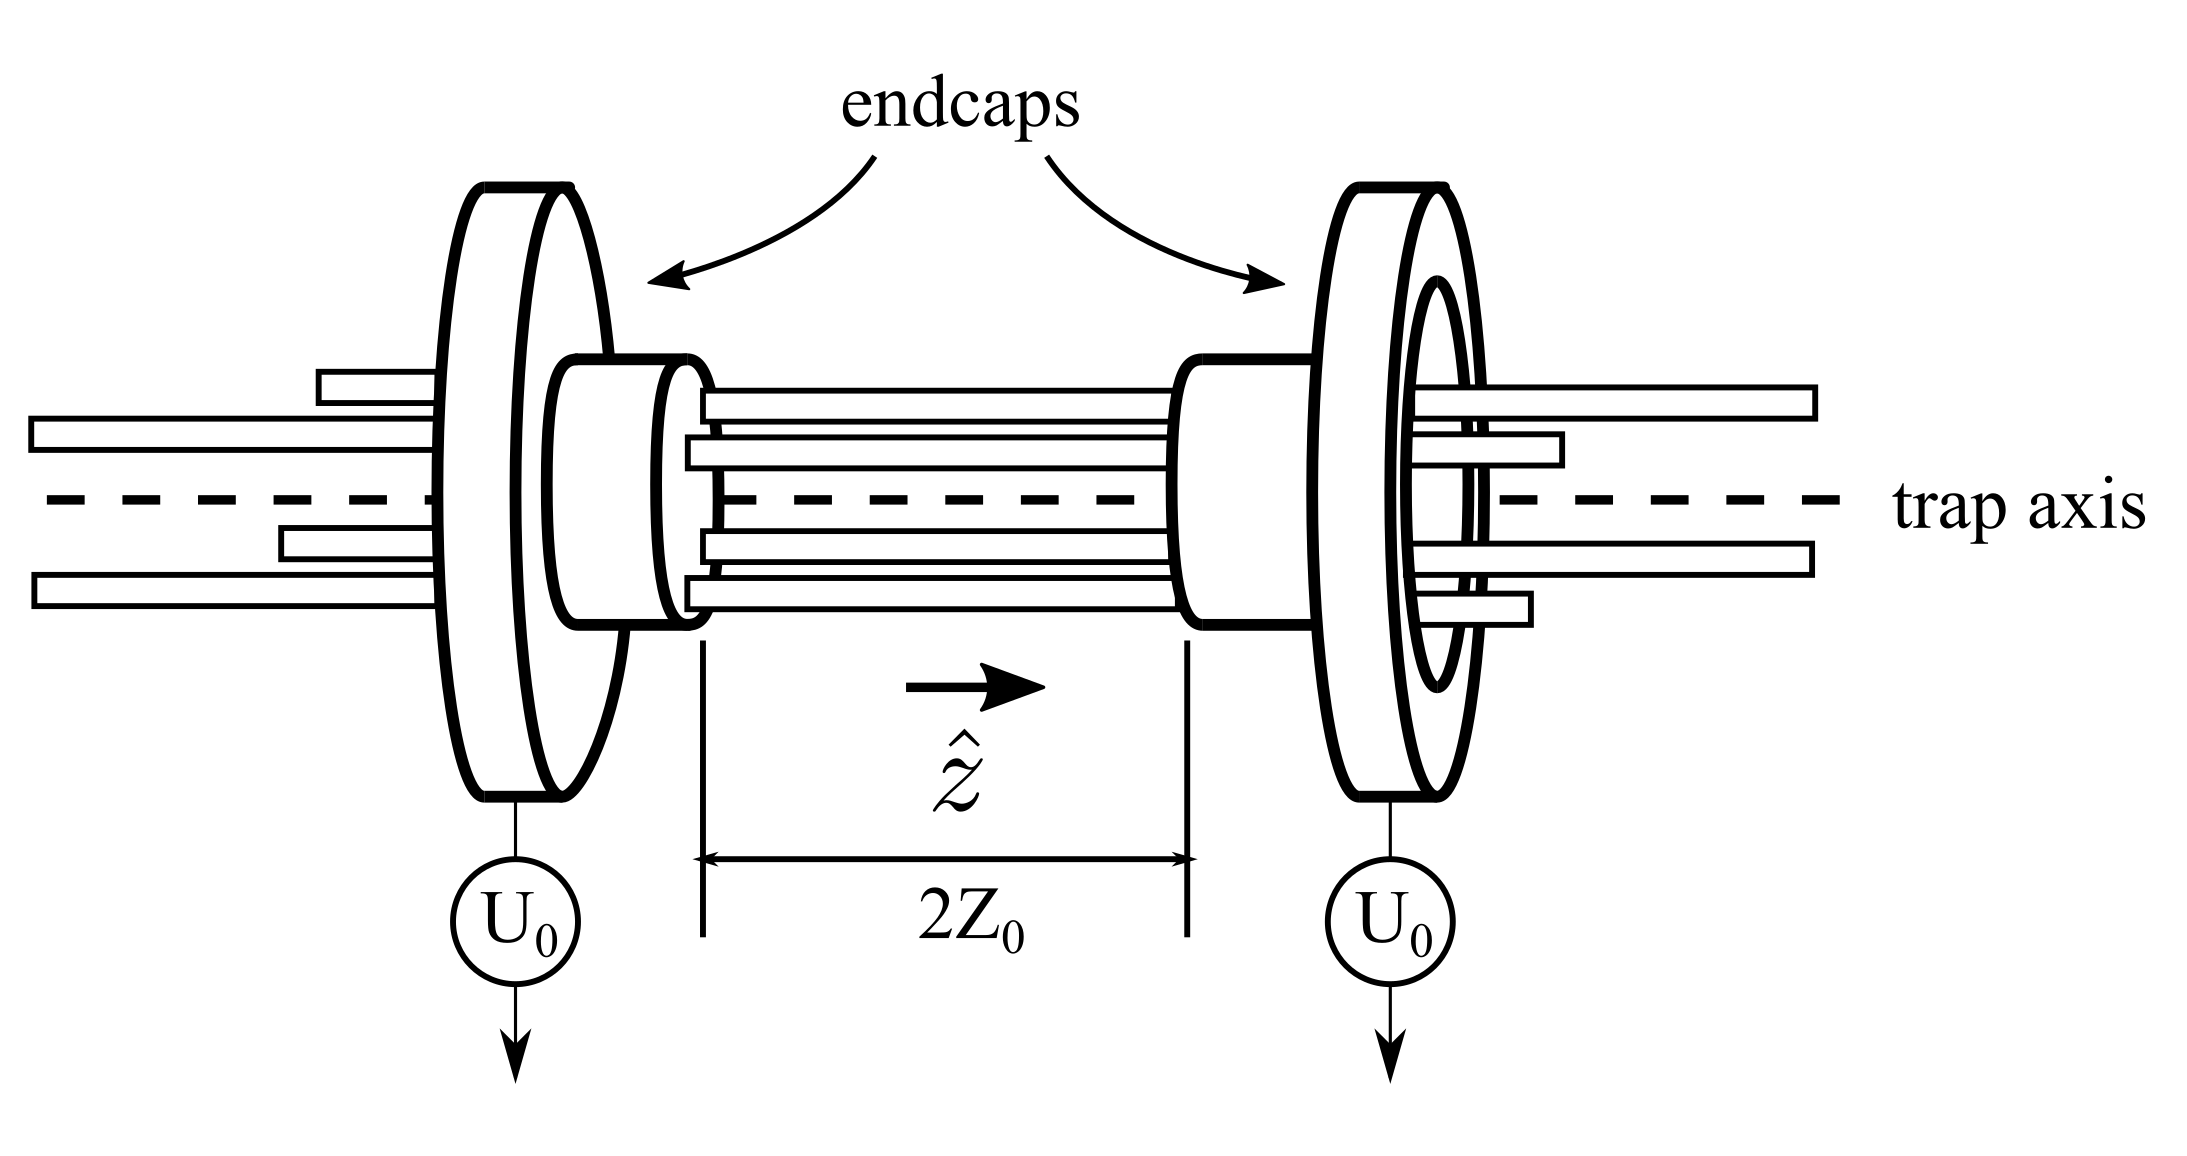
\includegraphics[width = 0.98\columnwidth]{./theory/figure/figure1a.png}
			\caption{リニア型Paulトラップを横から見た図}
			\label{fig:figure1a}
		\end{center}
	\end{minipage}
	\begin{minipage}{0.5\linewidth}
		\begin{center}
			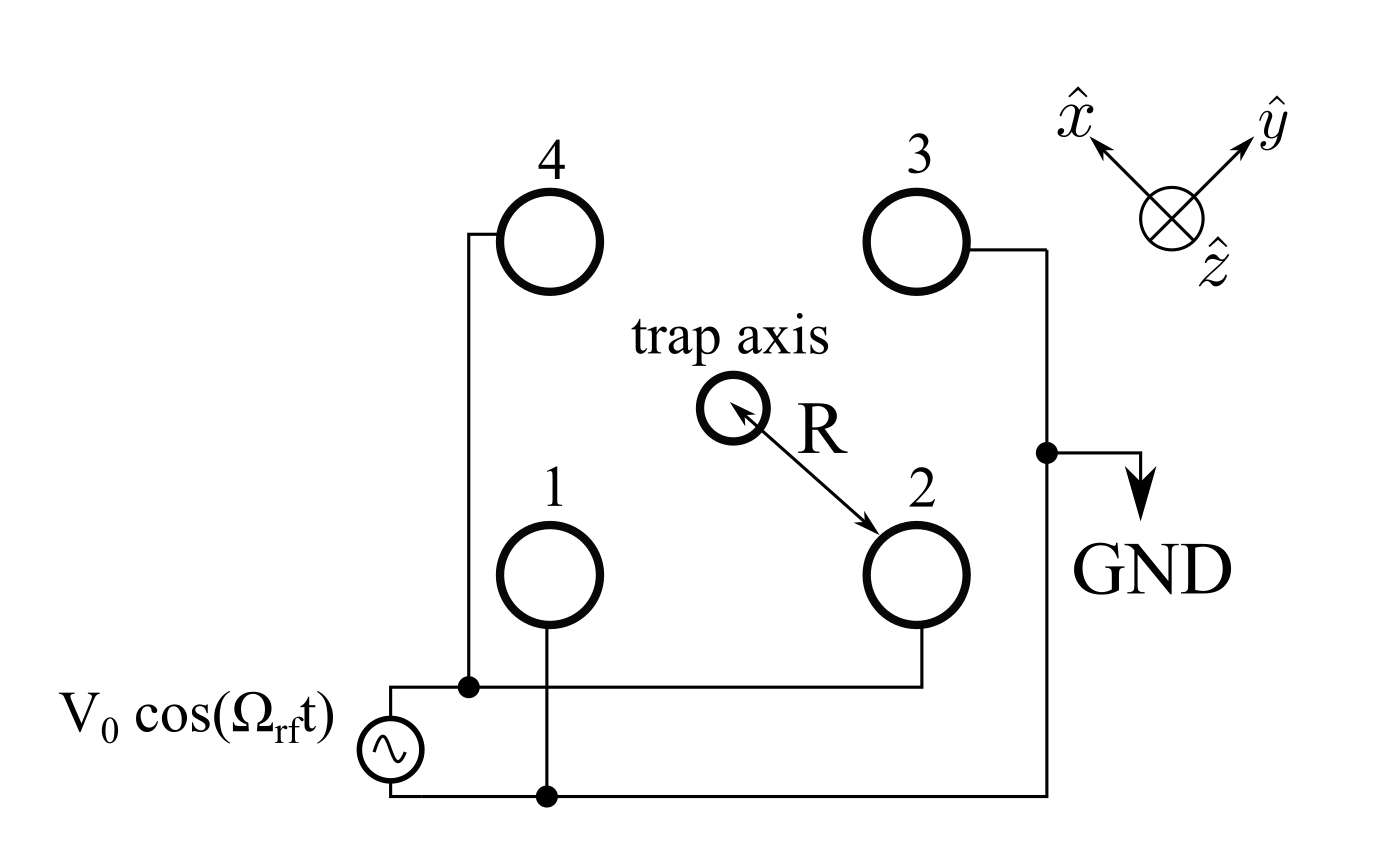
\includegraphics[width = 0.98\columnwidth]{./theory/figure/figure1b.png}
			\caption{リニア型Paulトラップをtrap axis方向から見た図}
			\label{fig:figure1b}
		\end{center}
	\end{minipage}
\end{figure}
%
\clearpage
%
1と3の電極は接地させて,2と4の電極には$V_0\cos(\Omega_{\rm rf}t)$のrf電圧を印加する.このとき,trap axis上に発生する電場は,
\large
\begin{align}\label{eq:trapaxis_E}
\bm{E}(x,y,z,t) = &-V_0\left( \frac{x\hat{x} - y\hat{y}}{R^{\prime 2}}\right) \cos(\Omega_{\rm rf} t) - \frac{\kappa U_0}{Z^2_0}\left[ 2z\hat{z} - x\hat{x} - y\hat{y} \right]
\end{align}
\normalsize
と計算される.ここで,$\kappa$は電極の幾何学的形状で決まる因子である.また,Rはtrap axisと電極間の距離であり,R $\simeq$ R$^\prime$である.なお,電極が無限長の双曲線円筒である場合にR=R$^\prime$が成立する\cite{Berkeland_1998}.

\subsection{rf擬ポテンシャル\cite{URABE}}
非常に高い周波数$\Omega_{\rm rf}$で発振する電圧(rf電圧)をrf電極に印加したときにイオンの見るポテンシャルについて考える.rf電圧によるポテンシャルは時間依存性を持ち,イオンの閉じ込めを行う方向が切り替わる.イオンがポテンシャルの開いている方向に逃げないタイミングで,閉じ込めの力がはたらくポテンシャルの方向を切り替えることで,イオンの閉じ込めを可能としている.rf電場が空間的に均一に分布している場合には,rf電圧の1周期でイオンが受ける力は平均してゼロになる.これに対し,rf電場が空間的に不均一である場合には,イオンの受ける力がその位置に依存する.したがって,不均一な電場内で振動するイオンには,1周期で平均したときに力がはたらく.この力によるポテンシャルを有効ポテンシャル,あるいはrf擬ポテンシャルと呼び,以下の式で与えられる.
\large
\begin{align}\label{eq:eff_pot}
	\Phi_{\rm eff}(x,y,z) = \frac{e^2}{4m\Omega_{\rm rf}^2}|\bm{E}(x,y,z)|^2
\end{align}
\normalsize
ここで,$m$はイオンの質量,$e$は素電荷量である.
\subsection{イオンの運動\cite{Berkeland_1998}\cite{URABE}}
\Eq{trapaxis_E}の中で,質量$m$,電荷$e$の単一イオンが運動するとき,イオンはMathieu方程式
\large
\begin{align}
	\frac{{\rm d^2}r_i}{{\rm d}t^2} + [a_i + 2q_i \cos (\Omega_{\rm rf} t)]\frac{\Omega_{\rm rf}^2}{4}r_i = 0. \quad (i = x,y,z)
\end{align}
\normalsize
に従う.このとき,
\large
\begin{align}
a_x &= a_y = -\frac{1}{2}a_z = -\frac{4 e \kappa U_0}{mZ^2_0 \Omega_{\rm rf}^2} \\
q_x &= -q_y = \frac{2eV_0}{mR^{\prime 2}\Omega_{\rm rf}^2},  q_z = 0
\end{align}
\normalsize
である.断熱近似($|q_i| \ll 1$,$|a_i| \ll 1$)の近似を用いることでMathieu方程式の近似解
\large
\begin{align}\label{eq:kinjikai}
r_i(t) &\approx r_{1i}\cos(\omega_i t + \varphi_{Si}) \left[ 1 + \frac{q_i}{2}\cos(\Omega_{\rm rf} t)\right] 
\end{align}
\normalsize
が得られる.ここで,$\omega_i$は永年周波数と呼ばれ,
\large
\begin{align}
\omega_i \approx \frac{1}{2}\Omega_{\rm rf}\sqrt{a_i + \frac{1}{2}q^2_i}
\end{align}
\normalsize
と近似される.\Eq{kinjikai}よりイオンの運動を2つの運動に分けることができる.第一項目の運動は永年運動と呼ばれ,ゆっくりと振動を行う運動となる.第二項目の運動はマイクロ運動と呼ばれ,速く振動する運動である.なお.マイクロ運動による振動が有効ポテンシャルの起源となっている.このとき,永年運動に対する有効ポテンシャルは
\large
\begin{align}
\Phi_{\rm eff} = \frac{m}{2e}(\omega_x^2 x^2 + \omega_y^2 y^2)
\end{align}
\normalsize

である.2つのendcapに$U_0$のdc電圧を印加したときのdcポテンシャルは,
\large
\begin{align}
\Phi_{\rm DC} &= \frac{\kappa U_0}{2Z_0^2}(2z^2 - x^2 - y^2) \\
					&= \frac{m}{2e}\omega_z^2 \left(z^2 - \frac{x^2 + y^2}{2}\right)
\end{align}
\normalsize
と計算される.したがって,イオンの三次元のポテンシャルは
\large
\begin{align}\label{eq:3D_harmonic}
\Phi_{\rm eff} + \Phi_{\rm DC} = \frac{m}{2e}(\omega^{\prime 2}_{x} x^2 + \omega^{\prime 2}_{y} y^2 + \omega_z^2)
\end{align}
\normalsize
と表すことができる.ここで,
\large
\begin{align}
\omega^{\prime 2}_x = \sqrt{\omega_x^2 - \frac{\omega_z^2}{2}} \\
\omega^{\prime 2}_y = \sqrt{\omega_y^2 - \frac{\omega_z^2}{2}}
\end{align}
\normalsize
とおいている.リニア型Paultトラップでは,z軸上でrf電場が0となり一列に並ぶイオンにおいてz方向に関するマイクロ運動が発生しない.

\subsection{余剰マイクロ運動\cite{Berkeland_1998}}
実際の系において,導線のインダクタンスや長さの違いなどに代表される電極の非対称性が含まれていることから,浮遊電場が現れる.ここで浮遊電場を一様な静電界$\bm{E}_{\rm stray}$として考える.このときのMathieu方程式は
\large
\begin{align}\label{eq:stray_mathieu_eq}
	\frac{{\rm d^2}r_i}{{\rm d}t^2} + [a_i + 2q_i \cos (\Omega_{\rm rf} t)]\frac{\Omega_{\rm rf}^2}{4}r_i = \frac{e\vec{E}_{\rm stray}\cdot \hat{r}_i}{m}. \quad (i = x,y,z)
\end{align}
\normalsize
となり,非同次の微分方程式となる.断熱近似の近似を用いて,\Eq{stray_mathieu_eq}の近似解をもとめると,
\large
\begin{align}\label{eq:stray_mathieu_kai}
r_i(t) &\approx [r_{0i} + r_{1i}\cos(\omega_i t + \varphi_{Si})]\left[ 1 + \frac{q_i}{2}\cos(\Omega_{\rm rf} t)\right]  \\
r_{0i} &\approx \frac{4e \bm{E}_{\rm stray} \cdot \hat{r}_i}{m(a_i + 1/2 q^2_i)\Omega_{\rm rf}^2} \approx \frac{e \bm{E}_{\rm stray} \cdot \hat{r}_i}{m\omega_i^2}
\end{align}
\normalsize
と表すことができる.これより,$\bm{E}_{\rm stray}$の存在によって\Eq{kinjikai}と比較してイオンの位置が,$\bm{r}_0 = r_{0x}\hat{x} + r_{0y}\hat{y} + r_{0z}\hat{z}$だけ変位する.このとき,$\hat{r}_i$に沿って,
\large
\begin{align}
r_{0i}\frac{q_i}{2} \cos(\Omega_{\rm rf}t)
\end{align}
\normalsize
の運動が発現する.これを余剰マイクロ運動と呼び,永年運動から派生するマイクロ運動とは区別して扱う.余剰マイクロ運動は浮遊電場の存在によって,dcポテンシャルの鞍点とrf擬ポテンシャルのnode点が一致しなくなることで発生する.また,rf電圧によって駆動されるため,レーザー冷却による冷却ができない.余剰マイクロ運動によって,
\begin{itemize}
\item イオンの光吸収スペクトルが変調されて,サイドバンド冷却が効率的に行えなくなる.
\item 遷移周波数のシフトにより,ACシュタルクシフトや二次のドップラーシフトが大きくなり,光周波数標準の精度に大きく影響を及ぼす.
\item rf加熱によって,イオンの運動状態が加熱されてしまう.
\end{itemize}
などの悪影響を受ける\cite{Timm_2015}.補正dc電圧を印加することで浮遊電場$\bm{E}_{\rm stray}$を打ち消すことで,余剰マイクロ運動を抑える必要がある.

\section{プレーナー型Paulトラップ}
プレーナー型Paulトラップは立体的な構造を持つPaulトラップの電極が同一平面上に配置された構造を持つ(\Fig{3D_to_2D}).プレーナートラップ型Paulトラップは単にプレーナートラップとも呼ばれる.プレーナートラップは立体的な構造を持つPaulトラップと比較して,電極構造に微細加工技術を施すことができることから,集積化に有利である.このことから,多くのプレーナートラップを並べて,その間でイオンの輸送を行うことで量子情報処理を行う,QCCD(Quantum Charge-Coupled Device)方式の提案\cite{Kielpinski_2002}がなされている.その反面,y方向におけるイオンを閉じ込めるポテンシャルが浅く,また,プレーナートラップ表面に垂直なレーザーを照射ができない等の問題も存在する.
\begin{figure}[h]
	\begin{center}
		\begin{minipage}{0.48\linewidth}
			\begin{center}
			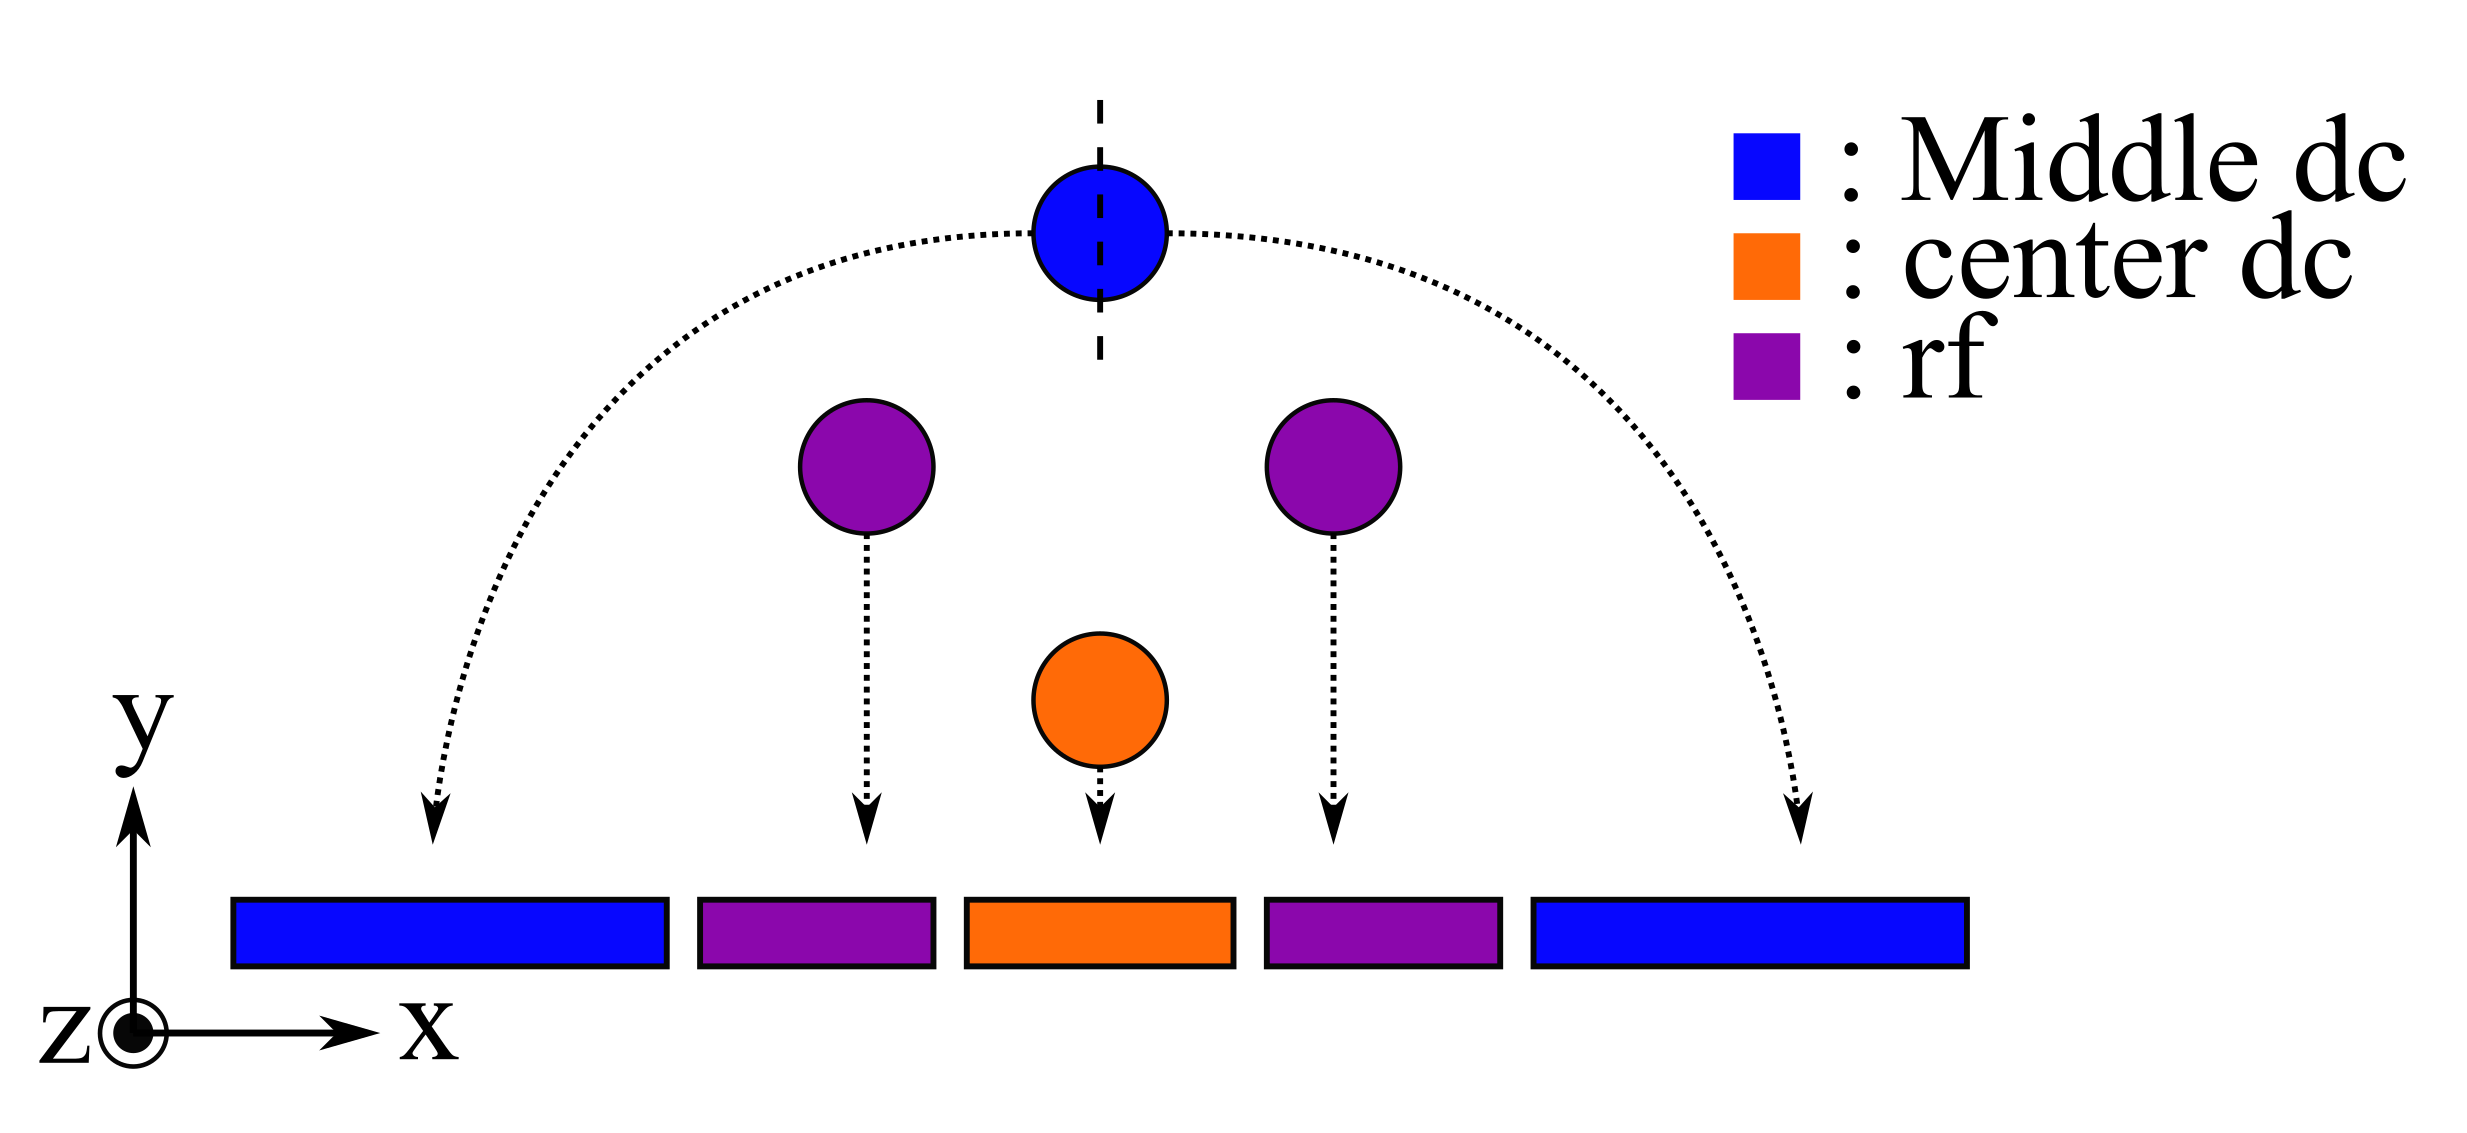
\includegraphics[width = 0.8\columnwidth]{./theory/figure/PaulTrap_3Dto2D_3DTrap.png}
			\end{center}
		\end{minipage}
		\begin{minipage}{0.48\linewidth}
			\begin{center}
			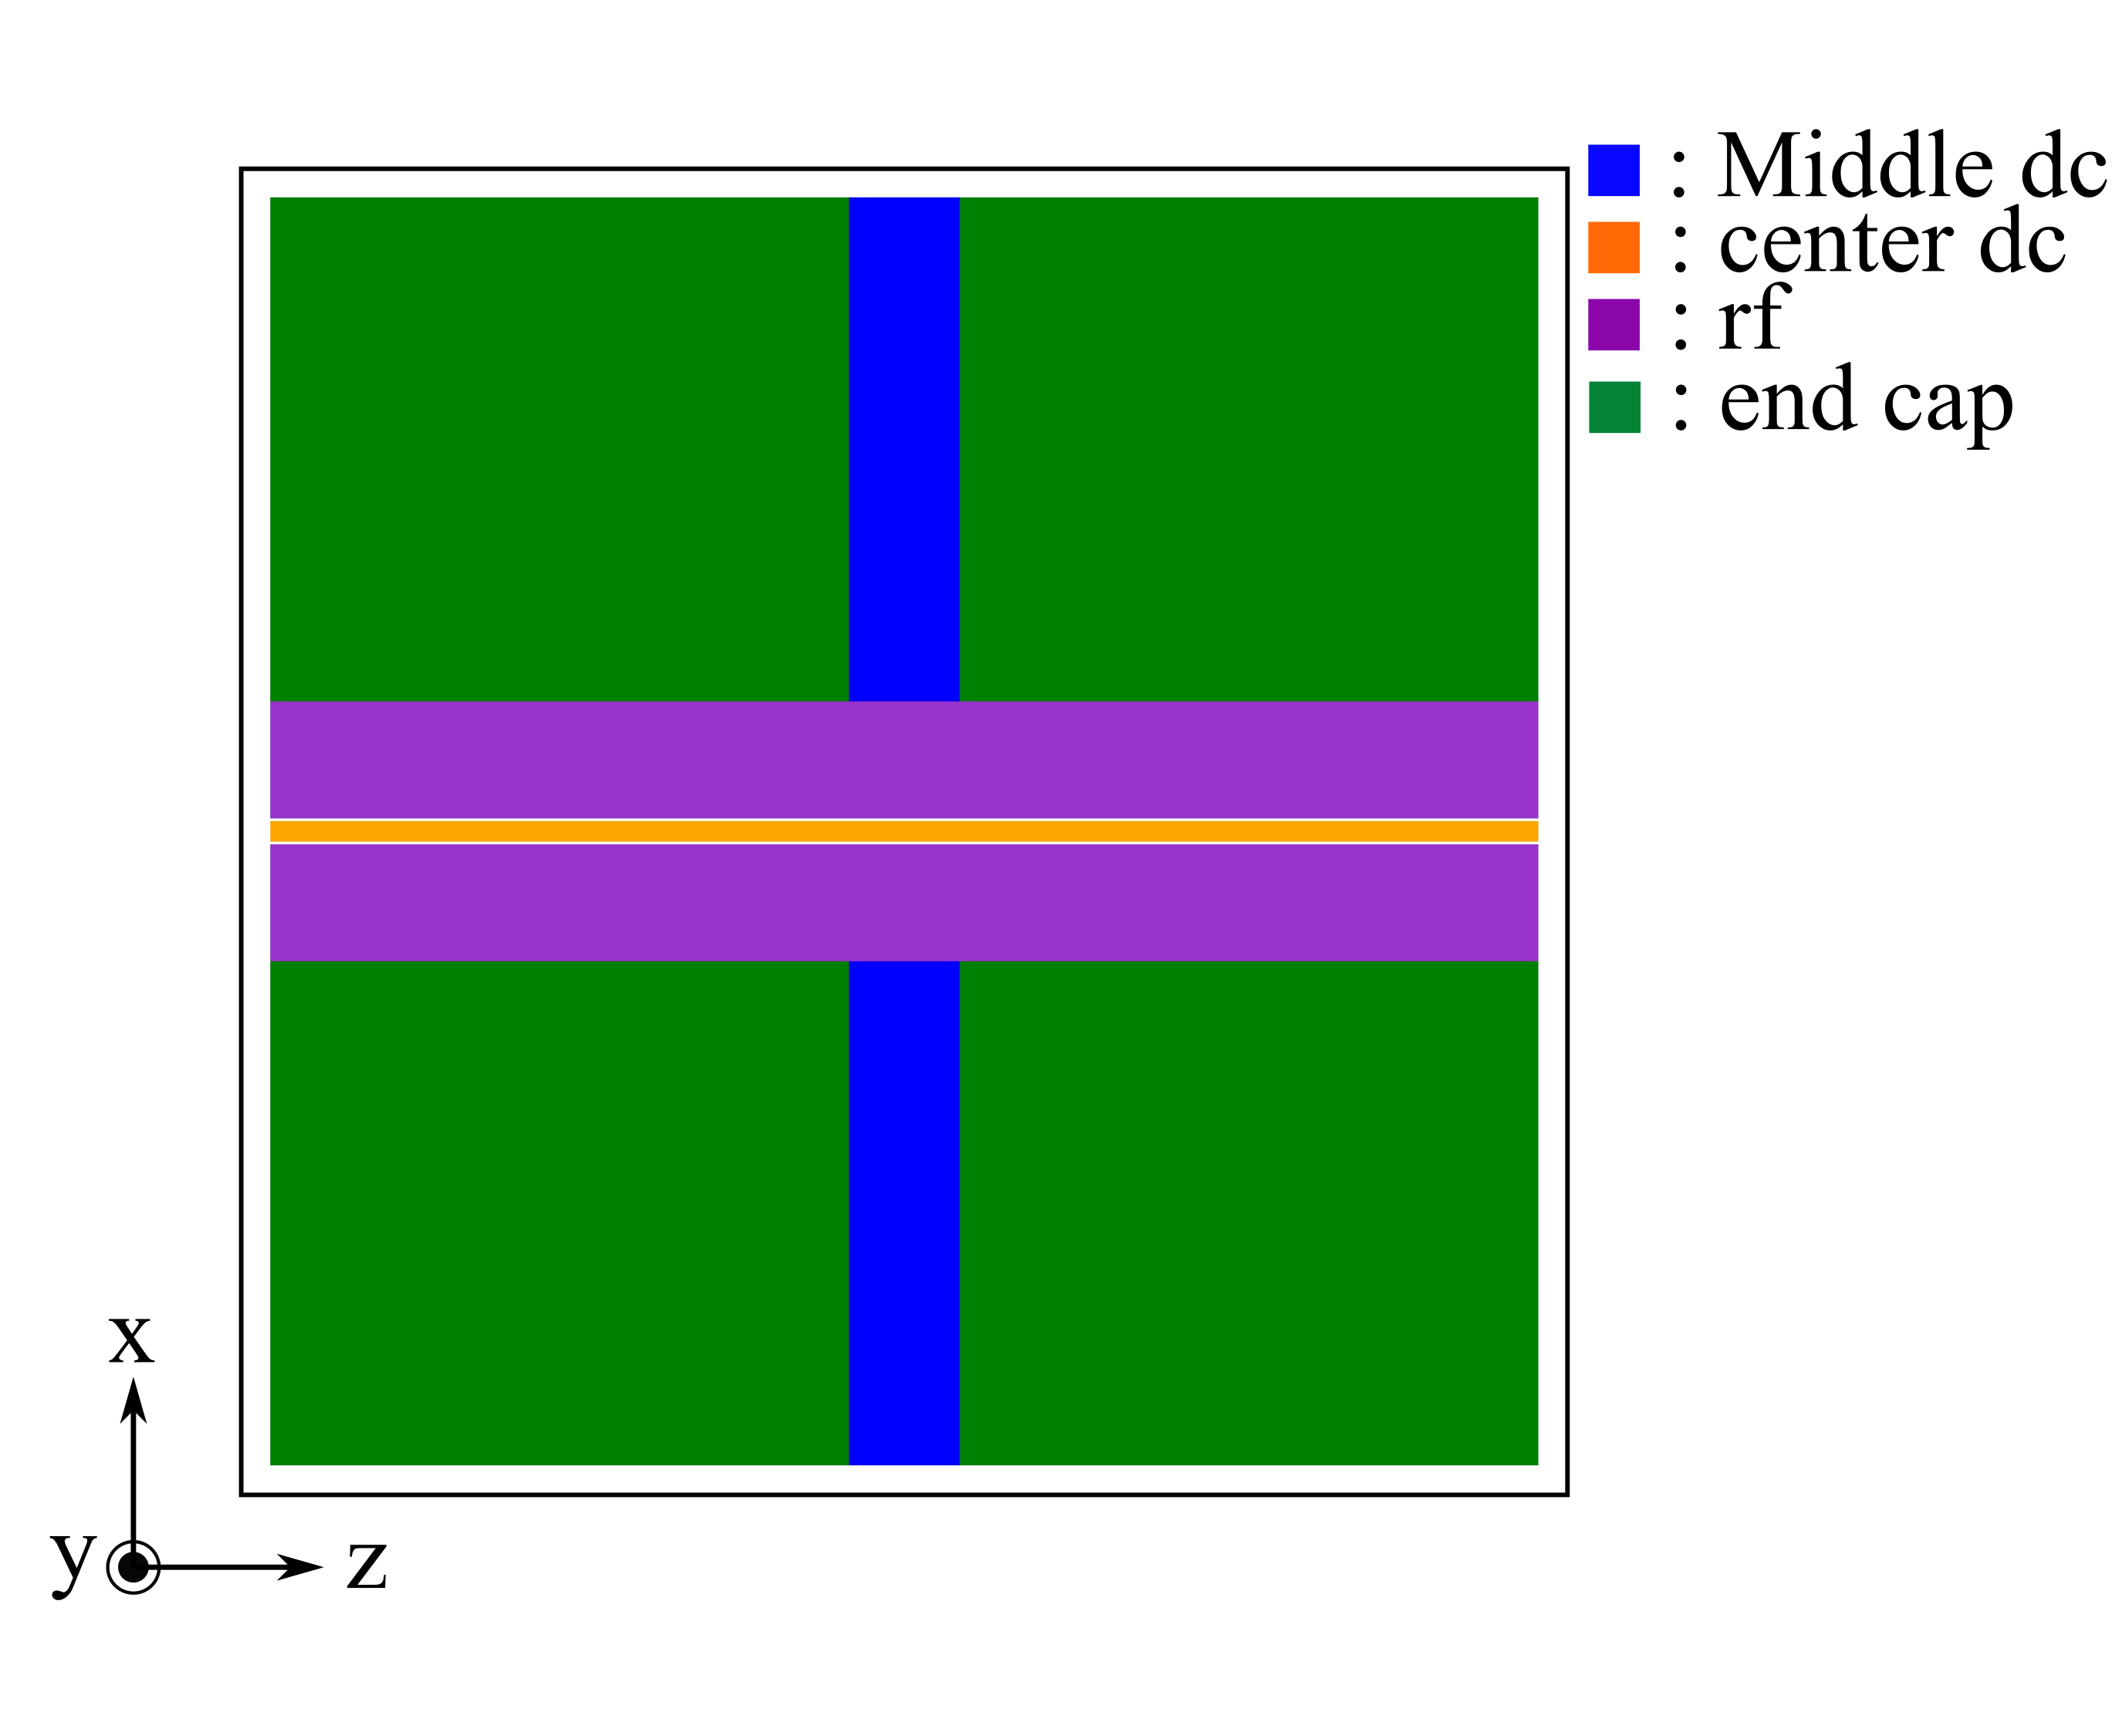
\includegraphics[width = 0.8\columnwidth]{./theory/figure/PaulTrap_3Dto2D_2DTrap.png}
			\end{center}
		\end{minipage}
	\end{center}
	\caption{リニア型Paulトラップとプレーナー型Paulトラップの各電極の対応関係}
	\label{fig:3D_to_2D}
\end{figure}

\subsection{プレーナートラップの仕様}
\Fig{Named_PlanerTrap}に本研究で用いるプレーナートラップの電極モデルを示す.

\begin{figure}[h]
	\begin{center}
		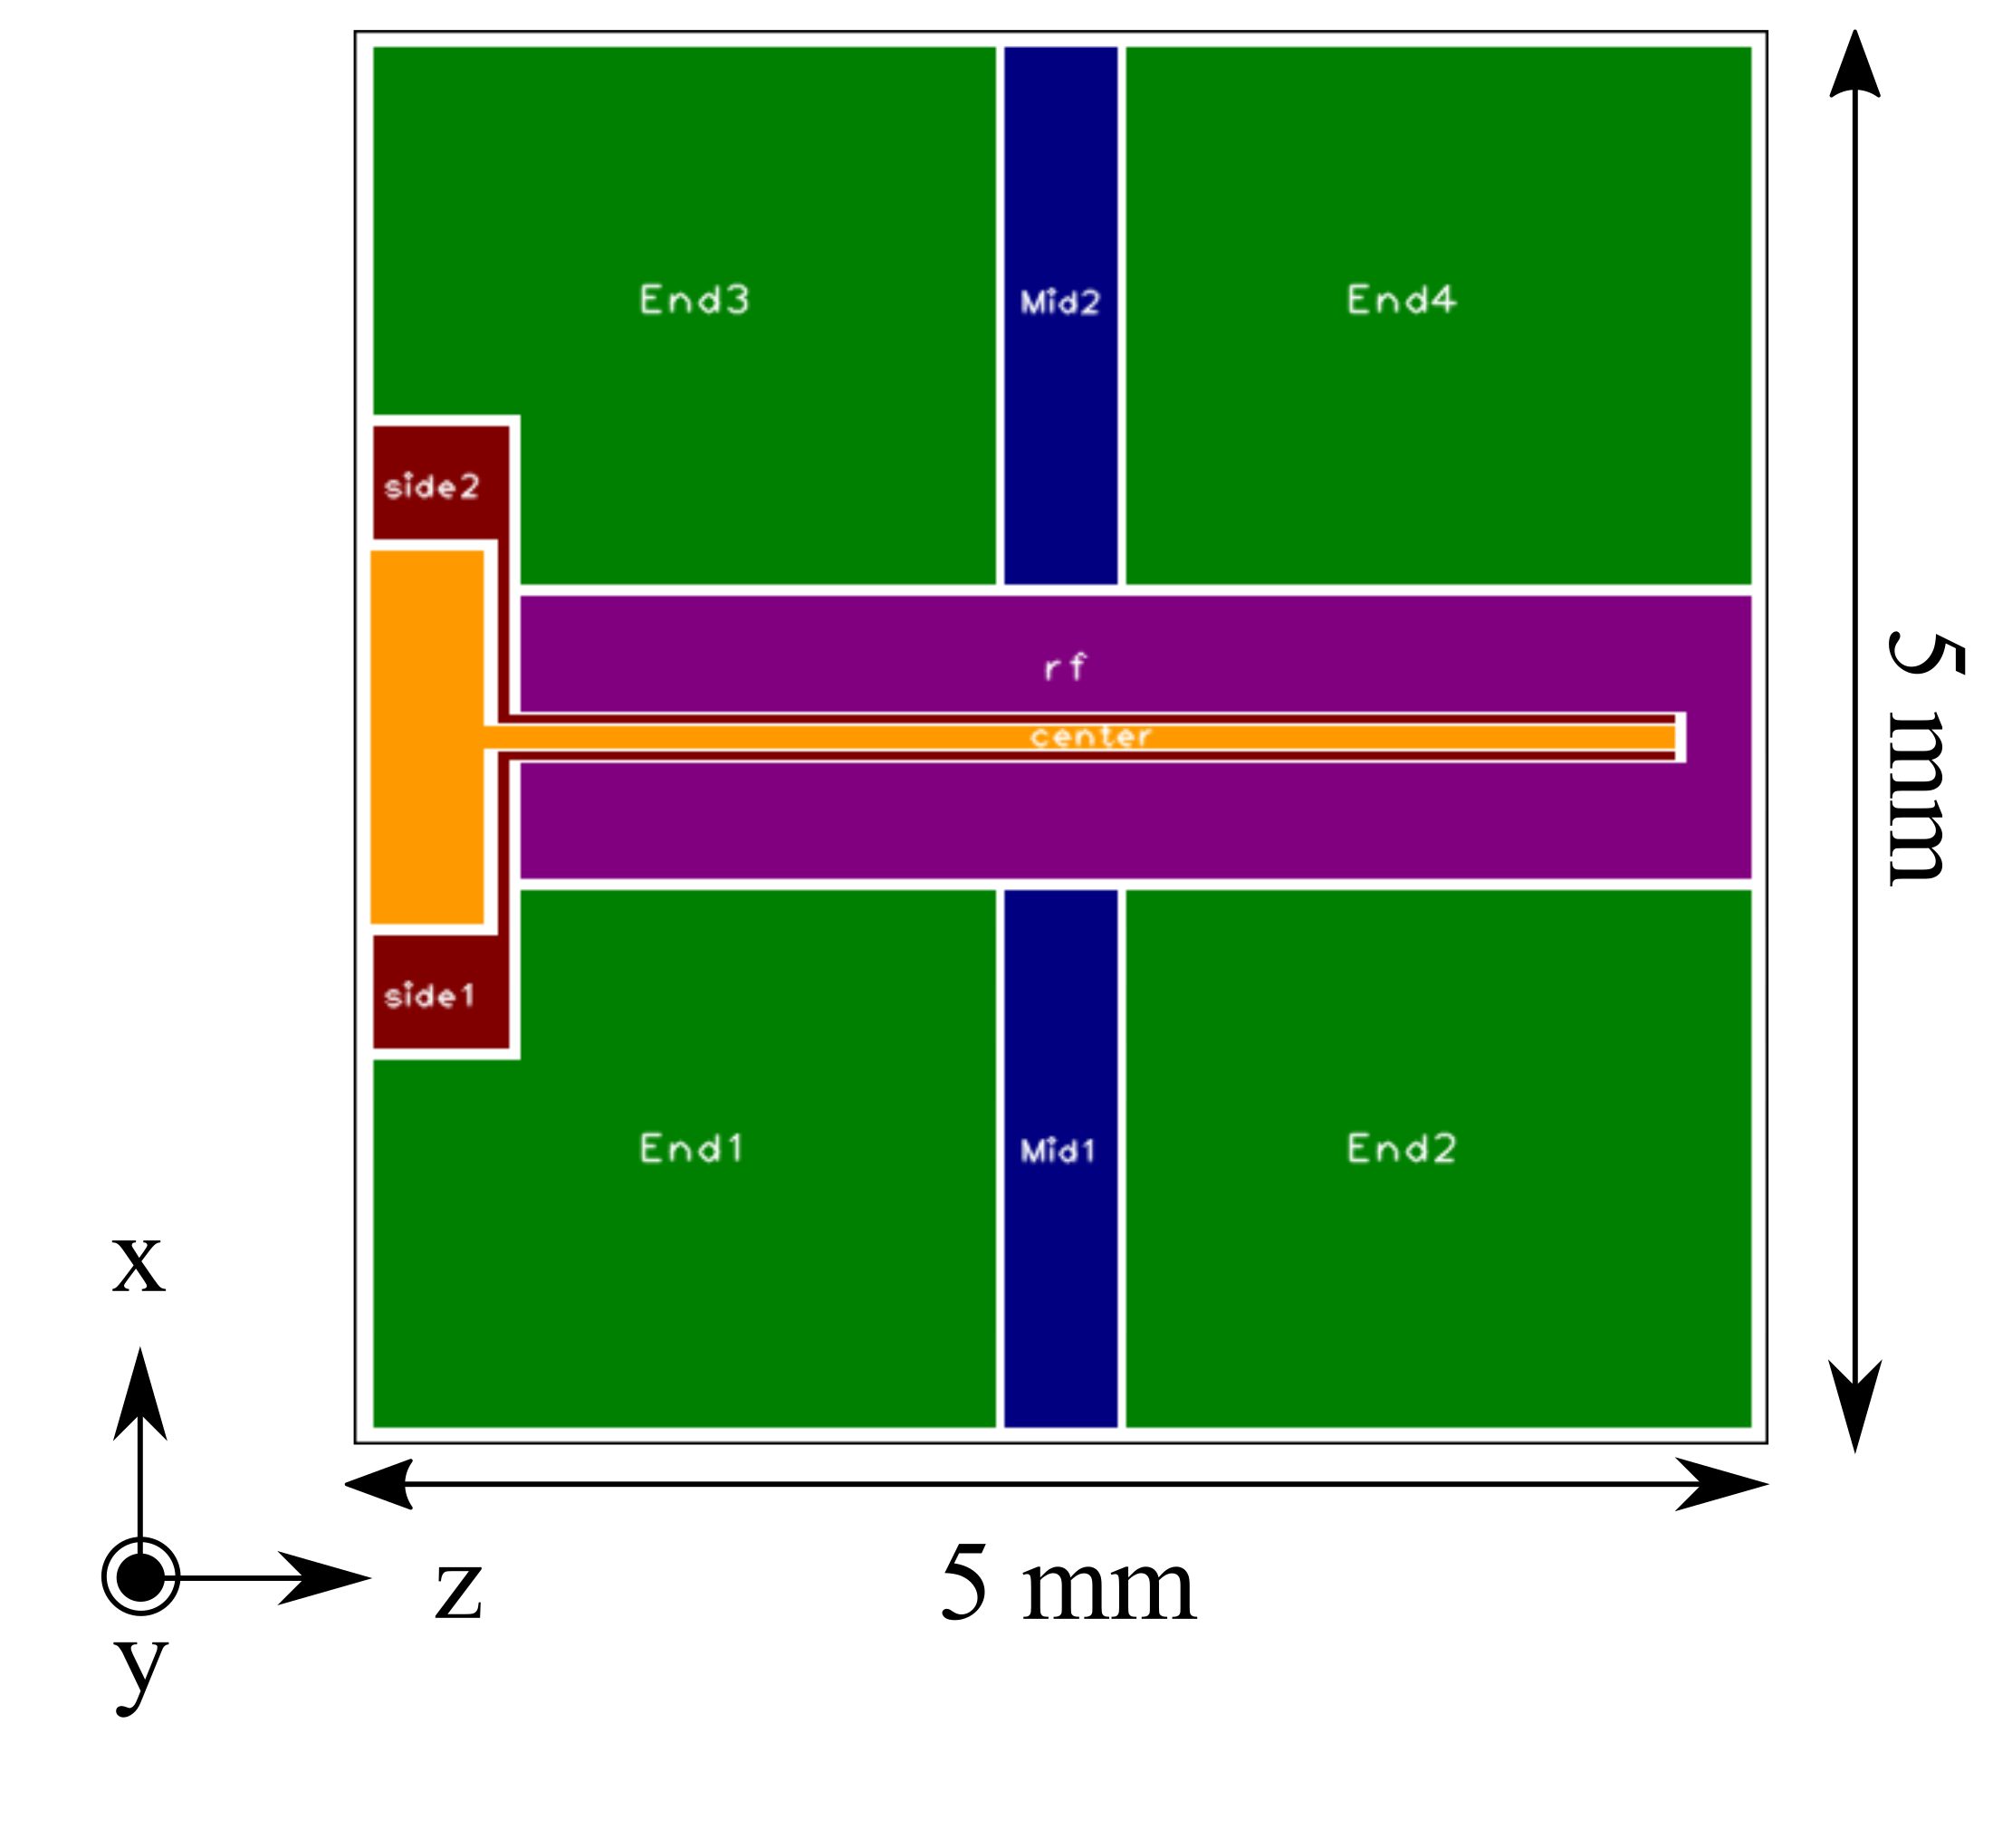
\includegraphics[width = 0.5\linewidth]{./theory/figure/named_electrode.png}
		\caption{本実験で使用するプレーナー型Paulトラップの電極モデル}
		\label{fig:Named_PlanerTrap}
	\end{center}
\end{figure}

\Fig{Named_PlanerTrap}に示される各電極にはそれぞれ役割がある.
\begin{description}
\item[rf電極] x, y方向の閉じ込めを行う.理論的にはz方向に対する閉じ込めの働きは持たない.
\item[End電極] 主にy, z方向の閉じ込めを行う.基本的にはz軸に関して向かい合ったEnd電極を一組として考える.2つの組に分けられるEnd電極に印加するdc電圧の比率を変化させることでdcポテンシャルの極小値を制御することができる.
\item[middle電極] End電極よりも低いdc電圧を印加することでz方向にdcポテンシャルの極小値を形成する.x方向に関してmiddle電極の電圧比を変化させることでdcポテンシャルの極小値を制御することでできるため,x方向におけるイオンの余剰マイクロ運動の抑制に使用する.通常,2つのmiddle電極には同じ電圧を印加する.
\item[center電極] y方向の閉じ込めの働きをする.正のy方向へ作用するため,y方向のdcポテンシャルの極小値はEnd電極とcenter電極の電圧比によって決定される.また,center電極にはrf電圧の印加を可能としている.これにより二列配列イオンの捕獲を可能としている.二列配列イオンの列間距離$d$はrf電極に印加するrf電圧の振幅とcenter-rf電圧に印加するrf電圧の振幅の比率$R$によって制御することができる.
\item[side電極] middle電極よりもイオン捕獲位置に近い位置に配置されていることから,x, y方向に存在するイオンの余剰マイクロ運動の抑制のために使用する.middle電極と同様に通常では2つのside電極には同じ電圧を印加する.
\end{description}

\subsection{矩形電極が作る静電ポテンシャル}
プレーナートラップ全体として形成するポテンシャルを計算するにあたり,まず任意の矩形電極に電圧$V$を印加したときに空間中のある点に形成する静電ポテンシャルの求め方を記述する.
\begin{figure}[h]
	\begin{center}
		
\includegraphics[width = 0.5\linewidth]{./theory/figure/Potential_of_rect-electrode.png}
		\caption{$(z_1,x_1),(z_2,x_2)$で指定される矩形が任意の点$(x,y,z)$に形成する静電ポテンシャル}
		\label{fig:Potential_from_rect-electrode}
	\end{center}
\end{figure}

\Fig{Potential_from_rect-electrode}に示すような矩形電極がy=0の平面に存在し,対向する頂点の座標が$(z_1, x_1), (z_2, x_2)$で与えられるとき($z_1 < z_2, x_1 < x_2$),$V$の電圧を印加された矩形電極が空間中のある点$(x,y,z)$に形成する静電ポテンシャル$\phi(x,y,z)$は以下のように計算することができる\cite{House_2008}.
\begin{align}\label{eq:rectangle_electrode}
	\phi(x,y,z) = \frac{V}{2\pi} \left\lbrace \arctan \left[ \frac{(x_2 - x)(z_2 - z)}{y\sqrt{y^2 + (x_2 - x)^2 + (z_2 - z)^2}}\right] - \arctan \left[ \frac{(x_1 - x)(z_2 - z)}{y\sqrt{y^2 + (x_1 - x)^2 + (z_2 - z)^2}} \right]  \right.  \notag \\ 
	\left. -\arctan \left[ \frac{(x_2 - x)(z_1 - z)}{y\sqrt{y^2 + (x_2 - x)^2 + (z_1 - z)^2}}\right] + \arctan \left[ \frac{(x_1 - x)(z_1 - z)}{y\sqrt{y^2 + (x_1 - x)^2 + (z_1 - z)^2}} \right]  \right\rbrace 
\end{align}

したがって,プレーナートラップ全体が作る静電ポテンシャルは,\Eq{rectangle_electrode}より各電極が形成する静電ポテンシャルの重ね合わせによって計算することができる.

%\section{イオンの平衡位置}

\section{レーザー冷却\cite{URABE}\cite{Wineland_1979}}
\begin{figure}[h]
	\begin{minipage}{0.5\linewidth}
		\begin{center}
			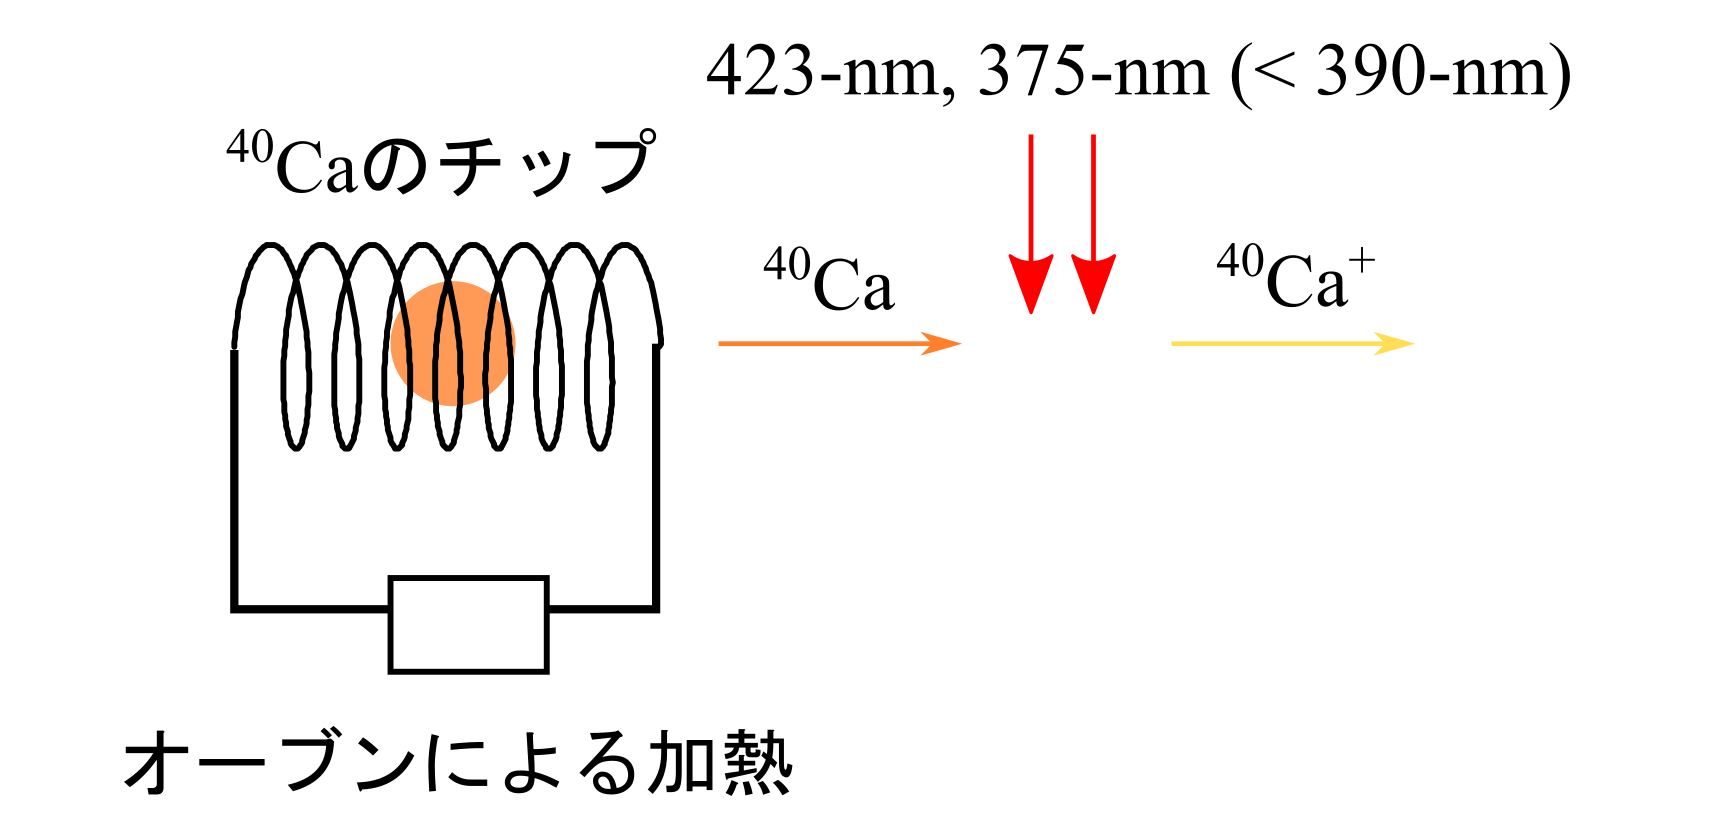
\includegraphics[width = 0.9\columnwidth]{./theory/figure/general_Ca+.png}
			\caption{$^{40}{\rm Ca}^{+}$の原子ビームを生成する過程}
			\label{fig:general_Ca+}
		\end{center}
	\end{minipage}
	\begin{minipage}{0.5\linewidth}
		\begin{center}
			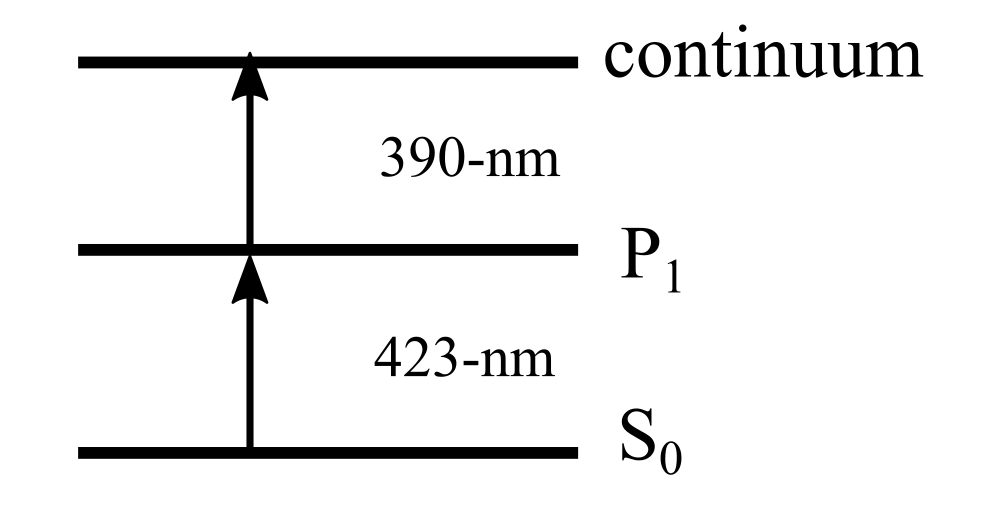
\includegraphics[width = 0.9\columnwidth]{./theory/figure/Ca_energy.png}
			\caption{$^{40}{\rm Ca}$のエネルギーバンド図}
			\label{fig:Ca_energy}
		\end{center}
	\end{minipage}
\end{figure}

%$^{40}{\rm Ca}^{+}$, $^{40}{\rm Ca}$
$^{40}{\rm Ca}^{+}$の捕獲を行うために,オーブンによって加熱されて,$^{40}{\rm Ca}$のチップから射出される原子ビームを光イオン化することでトラップ内に$^{40}{\rm Ca}^{+}$を生成する(\Fig{general_Ca+}).光イオン化を行うにあたり,\Fig{Ca_energy}に示すように,390-nm以下の波長をもつレーザーを照射することで電子が励起される.この過程で生成された$^{40}{\rm Ca}^{+}$は数千 K 程度の高温状態にあることからトラップすることができない.そこでイオンの温度を冷却する必要がある.イオンの冷却にはドップラー冷却やサイドバンド冷却などの手法が主に用いられる.そのほか,イオンの振動モードを一挙に冷却可能なE. I. T.冷却\cite{Lechner_2016}なども存在する.本研究においてイオンを捕獲する際に使用しているドップラー冷却について述べる. 


ドップラー冷却は,自然幅$\gamma$を持つ原子の二準位系を考えたときの共鳴周波数$\omega_0$に近い周波数を持つレーザーを原子に照射したときの光と原子の相互作用により生じる光の力を利用するものである.

\begin{figure}[h]
	\begin{minipage}{0.5\linewidth}
		\begin{center}
			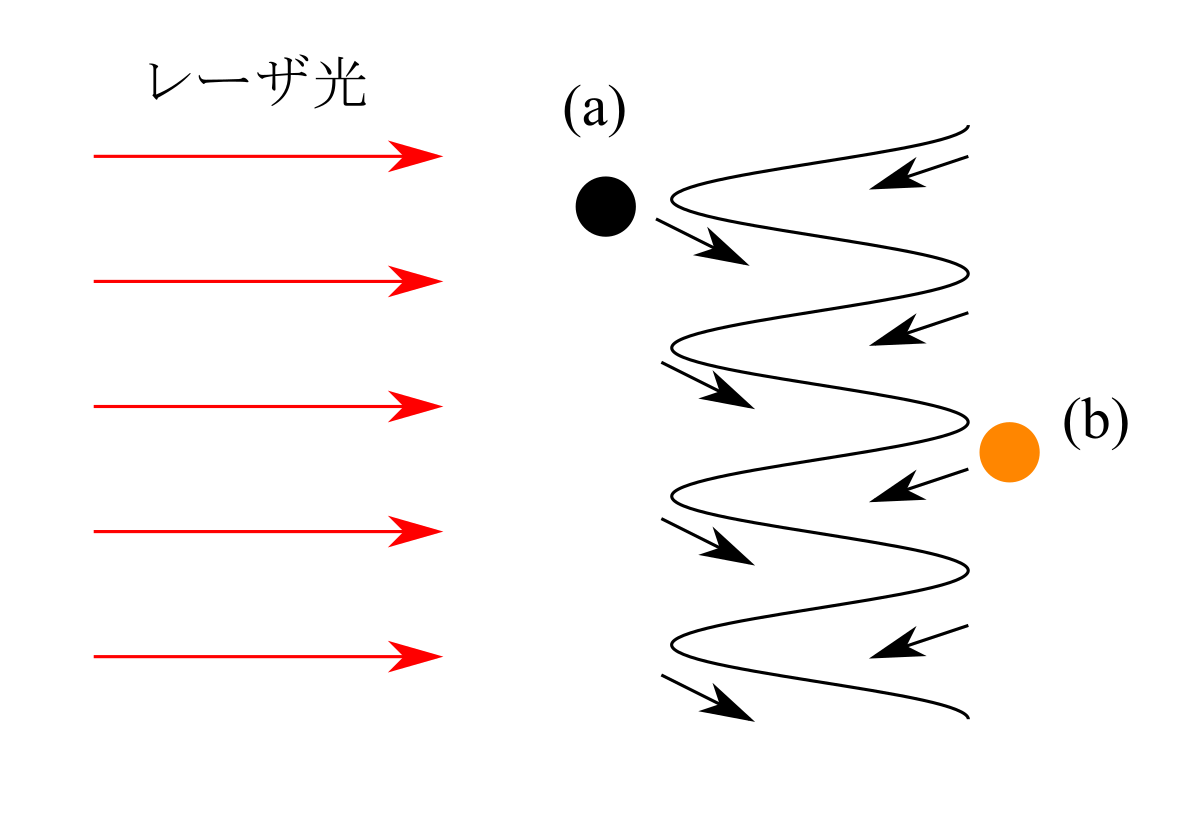
\includegraphics[width = 0.98\columnwidth]{./theory/figure/DopplerEffect.png}
			\caption{ドップラー効果}
			\label{fig:DopplerEffect}
		\end{center}
	\end{minipage}
	\begin{minipage}{0.5\linewidth}
			\begin{center}
				
\includegraphics[width = 0.98\columnwidth]{./theory/figure/cooling_spectrum.png}
				\caption{イオンの光吸収スペクトルとレーザーのスペクトル}
				\label{fig:cooling_spectrum}
			\end{center}
		\end{minipage}
\end{figure}

原子がある速度で運動している場合を考える.ここでは簡単のため,一次元での運動を考える.原子にレーザーを照射した場合に\Fig{DopplerEffect}(a),(b)の二つの場合が考えられる.また,照射するレーザーはある二準位系の共鳴周波数$\omega_0$から$\Delta\omega $だけ低い周波数$\omega_{\rm laser}$を持つとする(\Fig{cooling_spectrum}).すると,ドップラー効果によって,\Fig{DopplerEffect}(a)では原子が感じるレーザー光の周波数は$\omega_0$から離れ,反対に\Fig{DopplerEffect}(b)の場合には$\omega_0$に近くなる.つまり,レーザー光の進行方向に対向する場合に光の散乱が起こりやすくなる.レーザー光中の光子を放出する過程(\Fig{DopplerEffect}(a))では,光子を放出する方向は等方的であるため,運動量変化はゼロとなる.反対に,光子を吸収する過程(\Fig{DopplerEffect}(a))では,原子は運動量$\hbar \bm{k}$($\bm{k}$:光子の波数ベクトル)をもらう.したがって,1つの光子が吸収され放出される過程において,速度は平均で$\hbar \bm{k}/M$だけ変化することになる.このことからレーザー光の進行方向と原子の進む方向が対向する場合に,速度を低減させ,冷却の効果が現れる.ただし,光子の放出する過程においては加熱の効果が現れる.このとき,冷却に最適なレーザーの周波数は
\large
\begin{align}
\Delta \omega = - \frac{\gamma}{2}
\end{align}
\normalsize
であり,冷却限界温度$T_{\rm doppler}$は,
\large
\begin{align}
T_{\rm doppler} = \frac{\gamma}{4}\hbar
\end{align}
\normalsize
で与えられる.イオンの温度を数$\mu$Kまで冷却するためには吸収と放出を繰り返すための閉じたサイクルを必要とする.

\begin{figure}[h]
	\begin{center}
		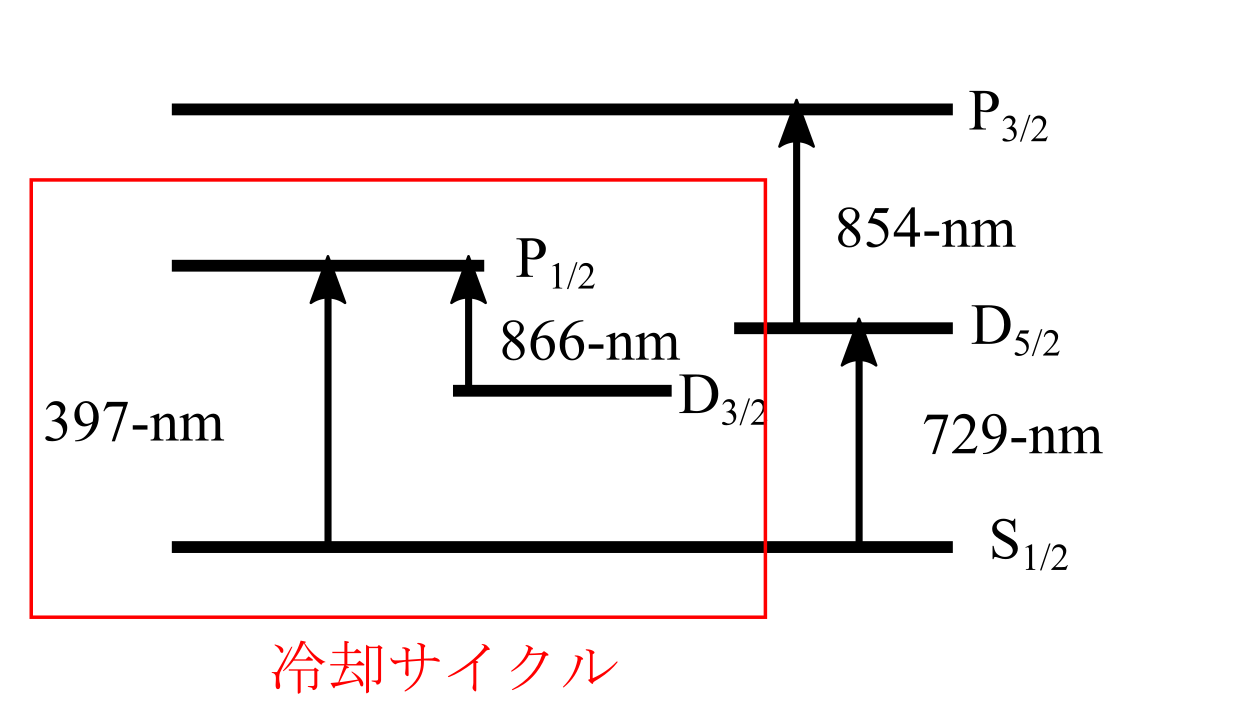
\includegraphics[width = 0.6\linewidth]{./theory/figure/Ca+_energy.png}
		\caption{$^{40}{\rm Ca}^+$のエネルギーバンド図}
		\label{fig:Ca+_energy}
	\end{center}
\end{figure}

\Fig{Ca+_energy}に$^{40}{\rm Ca}^{+}$のエネルギー準位図を示す.ドップラー冷却を行うサイクルを${\rm S}_{1/2} - {\rm P}_{1/2}$遷移で行い,397-nmのレーザーを用いて誘導吸収を引き起こす.$^{40}{\rm Ca}^{+}$の場合,${\rm P}_{1/2}$準位に励起されたイオンのうち,約94\%が${\rm S}_{1/2}$準位に遷移し,約6\%が${\rm D}_{3/2}$準位に遷移する.${\rm D}_{3/2}$は準安定準位であるため冷却効率が下がってしまう.そのため,${\rm S}_{1/2} - {\rm D}_{3/2}$遷移を引き起こすためのリポンプ用のレーザーとして866-nmの照射を行い,閉じた冷却サイクルの維持を図る.


\section{画像処理によるイオン捕獲位置と電場の算出}
OpenCVとNumpyを使って画像処理を行うことでイオンの位置と,イオンの位置における電場の算出を行う.ここでは画像処理の方法について述べる.
\subsection{ヒストグラムの正規化}
カメラでイオンの蛍光を撮像する際に,カメラの集光時間やピントおよび照射するレーザーの波長や位置などによって得られるイオン捕獲画像の輝度値のヒストグラムは変化する.輝度値が0に近い画素が多ければ画像は全体として暗く,255に近い画素が多ければ画像は全体として明るくなる.\Fig{ionimage}に示すイオン捕獲画像を例にヒストグラムの偏りを\Fig{hist}に示す.
\begin{figure}[h]
	\begin{center}
	\begin{minipage}{0.3\linewidth}
		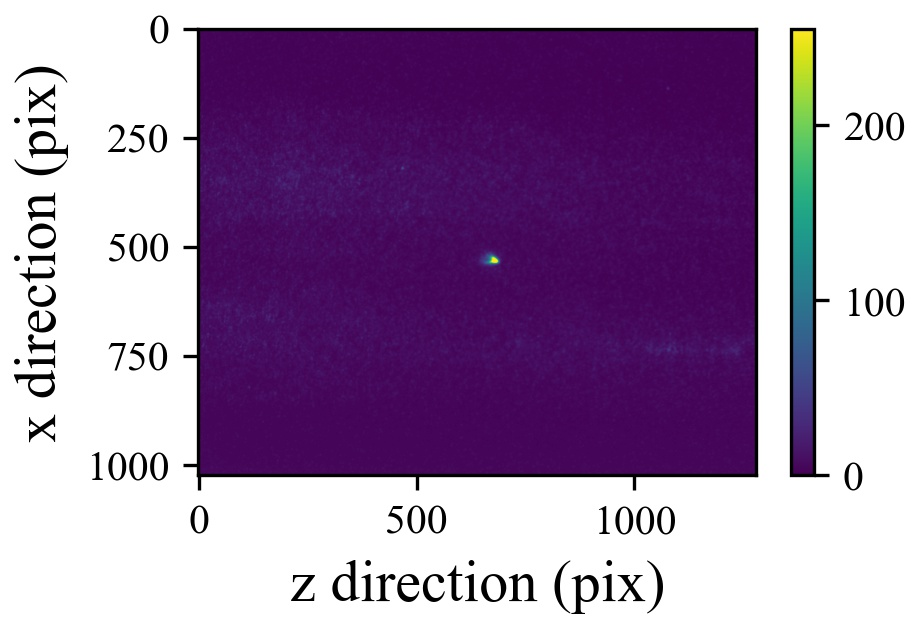
\includegraphics[width=0.98\columnwidth]{./theory/figure/5/image_0.jpg}
	\end{minipage}
	\begin{minipage}{0.3\linewidth}
		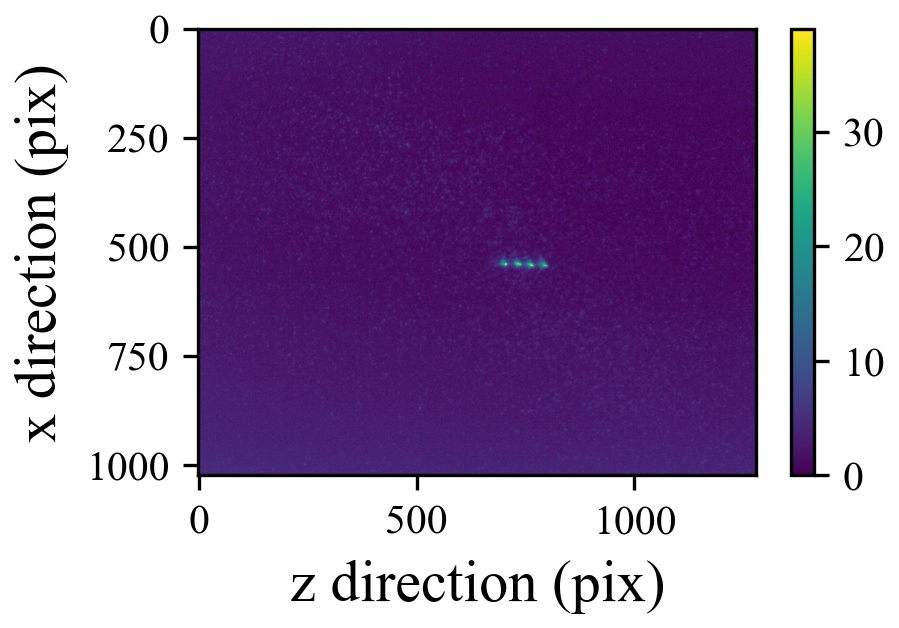
\includegraphics[width=0.98\columnwidth]{./theory/figure/5/image_1.jpg}
	\end{minipage}
	\begin{minipage}{0.3\linewidth}
		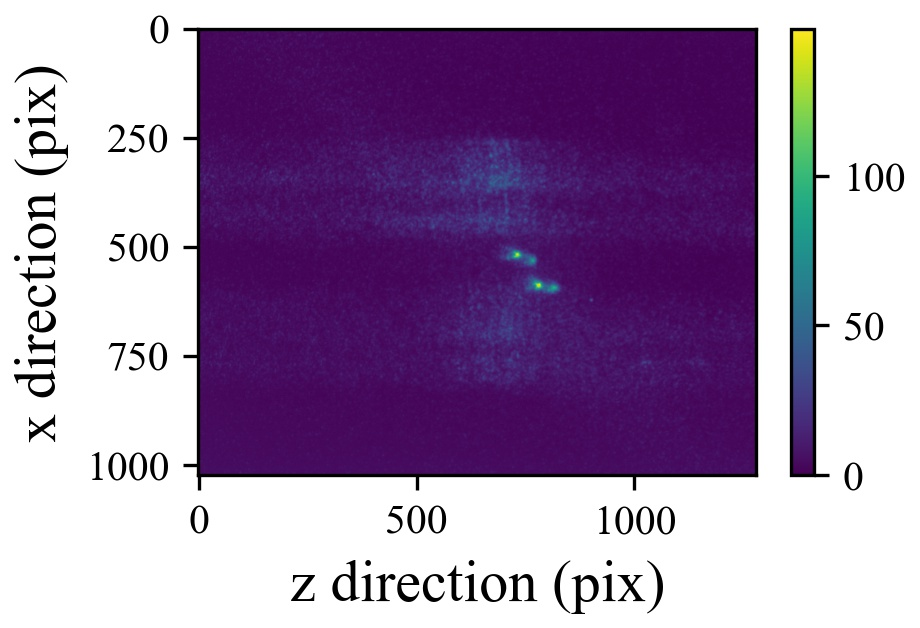
\includegraphics[width=0.98\columnwidth]{./theory/figure/5/image_2.jpg}
	\end{minipage}
	\end{center}
	\caption{集光系のピントおよびレーザー照射位置などが異なる場合のイオン捕獲画像}
	\label{fig:ionimage}
\end{figure}

\begin{figure}[h]
	\begin{center}
		\begin{minipage}{0.3\linewidth}
			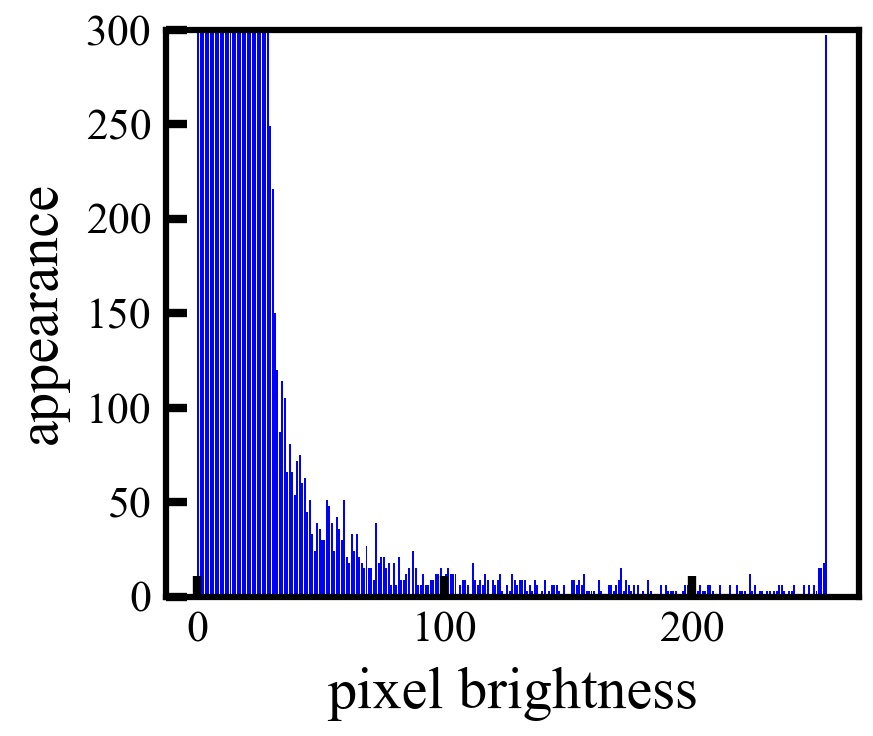
\includegraphics[width=0.98\columnwidth]{./theory/figure/5/hist_0.jpg}
		\end{minipage}
		\begin{minipage}{0.3\linewidth}
			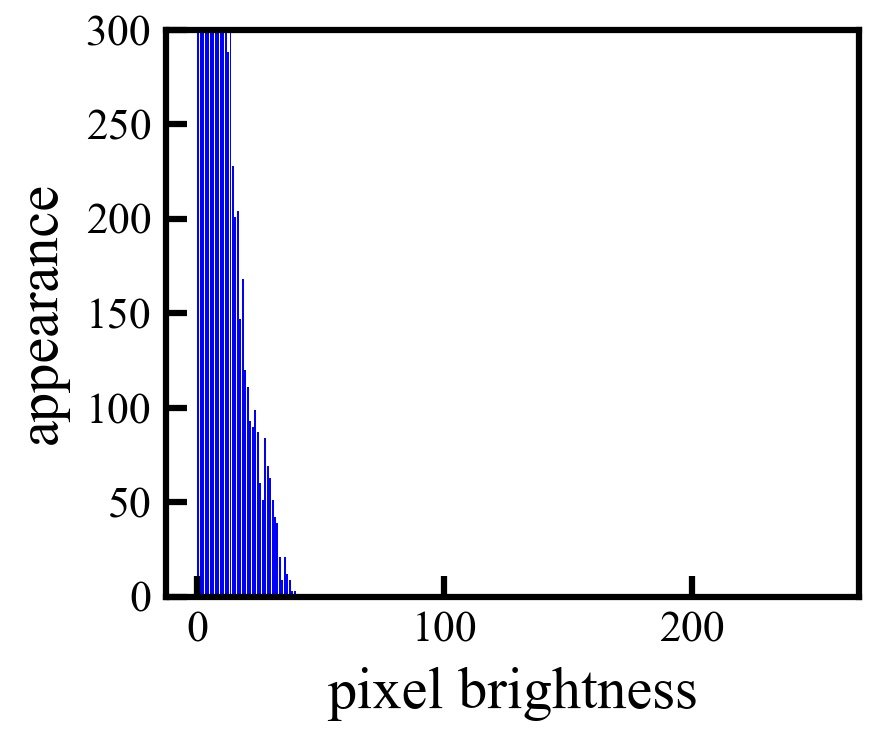
\includegraphics[width=0.98\columnwidth]{./theory/figure/5/hist_1.jpg}
		\end{minipage}
		\begin{minipage}{0.3\linewidth}
			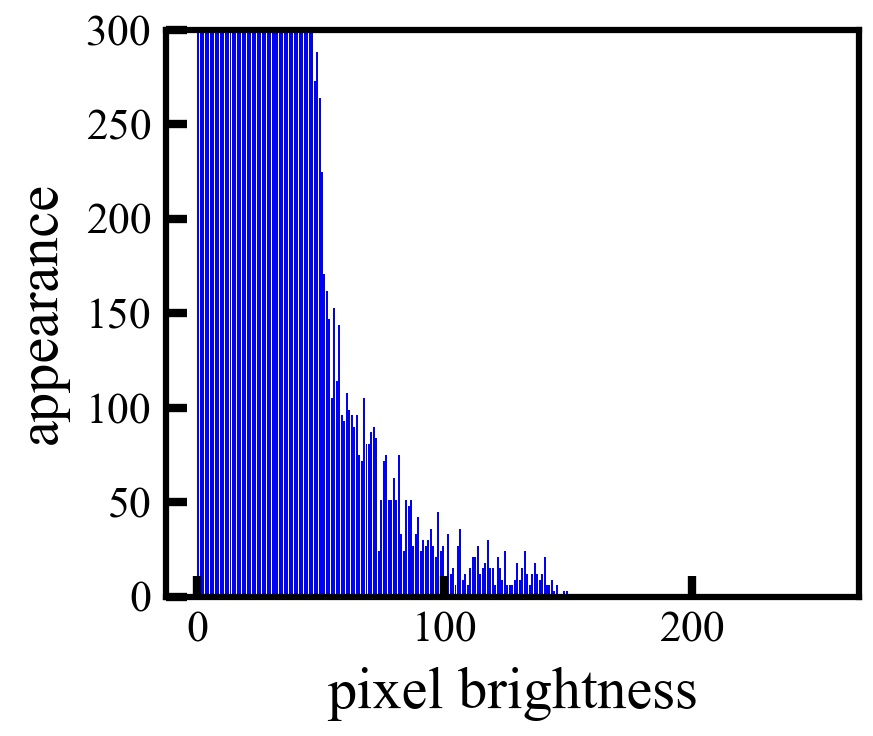
\includegraphics[width=0.98\columnwidth]{./theory/figure/5/hist_2.jpg}
		\end{minipage}
	\end{center}
	\caption{\Fig{ionimage}の各画像のピクセル輝度値のヒストグラム}
	\label{fig:hist}
\end{figure}

イオンの位置特定を行うに際し,二値化の処理のための閾値を定める.しかし,\Fig{hist}のように輝度値の偏りが各画像において異なっている場合,閾値を画像毎に変化させる必要がある.これを防ぐために濃度諧調変換と呼ばれるヒストグラムの正規化を行う.[c,d]の画素値を持つ画像を[a,b]のレンジに変換する式は次式で与えられる.

\large
\begin{align}\label{eq:GS_trans}
x_{\rm out} = 
\left\{ 
\begin{array}{ll}
	a & {\rm if} \ x_{\rm in} < c \\
	\frac{b-a}{d-c}(x_{\rm in}-c) + a & {\rm else \ if} \ c \leq x_{\rm in} < d \\
	b &{\rm else}
\end{array} \right.
\end{align}
\normalsize
ここでa,bは任意であり,cはある画像における輝度値の最小値,dは最大値とする.

\Fig{hist}に対して\Eq{GS_trans}を$a=0,b=255$として適用させると\Fig{norm_hist}となる.
\begin{figure}[h]
	\begin{center}
		\begin{minipage}{0.3\linewidth}
			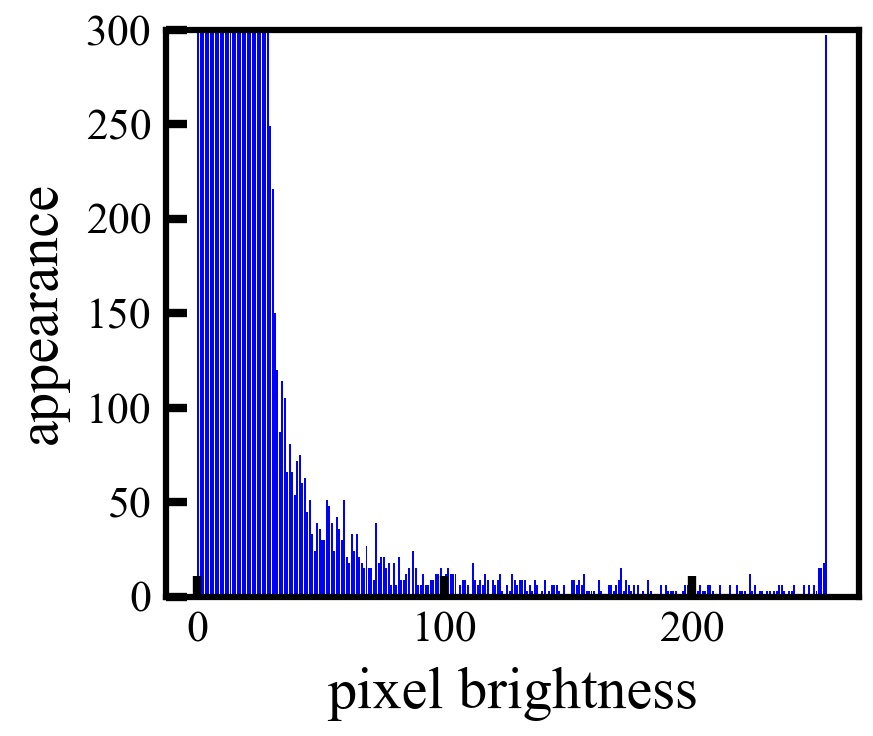
\includegraphics[width=0.98\columnwidth]{./theory/figure/5/norm_hist_0.jpg}
		\end{minipage}
		\begin{minipage}{0.3\linewidth}
			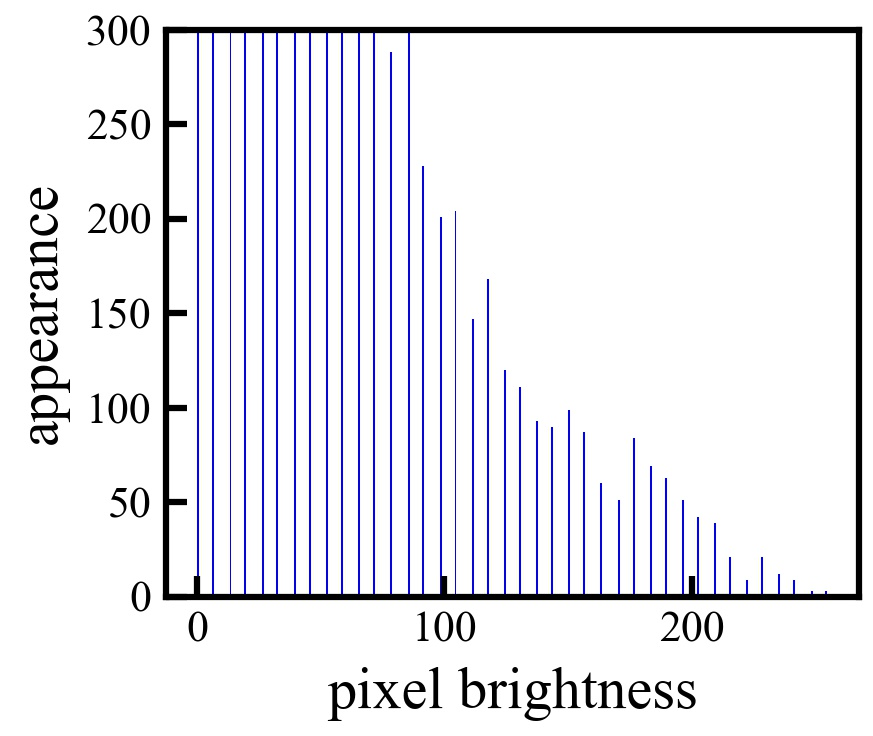
\includegraphics[width=0.98\columnwidth]{./theory/figure/5/norm_hist_1.jpg}
		\end{minipage}
		\begin{minipage}{0.3\linewidth}
			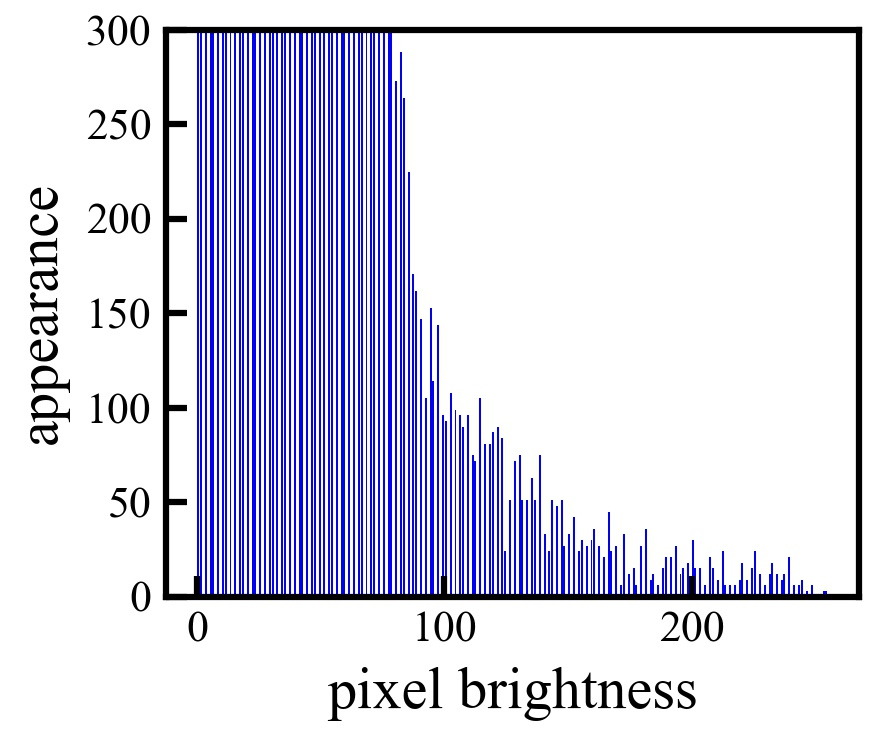
\includegraphics[width=0.98\columnwidth]{./theory/figure/5/norm_hist_2.jpg}
		\end{minipage}
	\end{center}
	\caption{\Fig{ionimage}の各画像のピクセル輝度値を正規化したときのヒストグラム}
	\label{fig:norm_hist}
\end{figure}

\subsection{二値化}
二値化とは,画像を特定の値を閾値として黒(=0)と白(=255)の2値で表現する方法である.二値化は次式で表される式を用いて変換される.
\large
\begin{align}\label{eq:binary_trans}
	x_{\rm out} = 
	\left\{ 
	\begin{array}{ll}
		0 & {\rm if} \ x_{\rm in} < {\rm threshold} \\
		255 & {\rm otherwise}
	\end{array} \right.
\end{align}
\normalsize
\Fig{thre_norm_hist}に\Eq{binary_trans}を${\rm threshold} = 128$として二値化を行ったときのヒストグラムを\Fig{binary_hist}に示す.
\begin{figure}[h]
	\begin{center}
		\begin{minipage}{0.3\linewidth}
			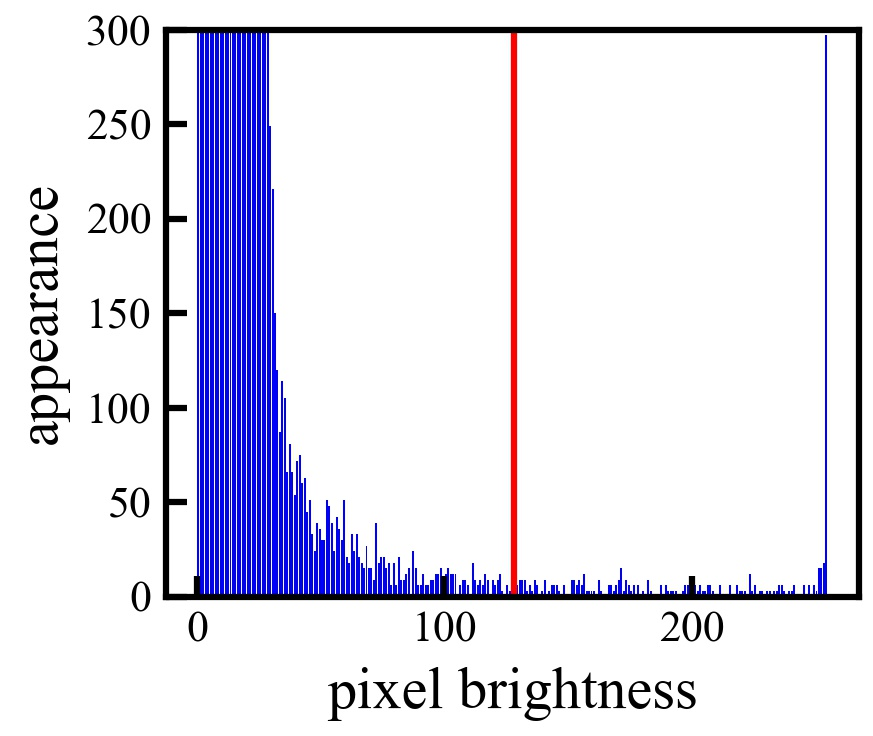
\includegraphics[width=0.98\columnwidth]{./theory/figure/5/thre_norm_hist_0.jpg}
		\end{minipage}
		\begin{minipage}{0.3\linewidth}
			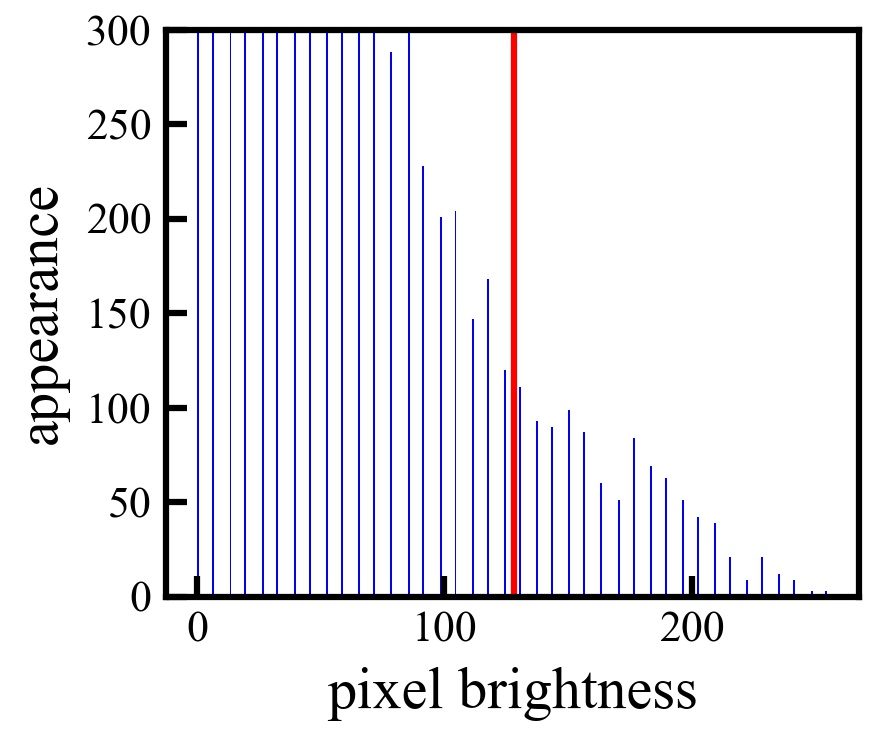
\includegraphics[width=0.98\columnwidth]{./theory/figure/5/thre_norm_hist_1.jpg}
		\end{minipage}
		\begin{minipage}{0.3\linewidth}
			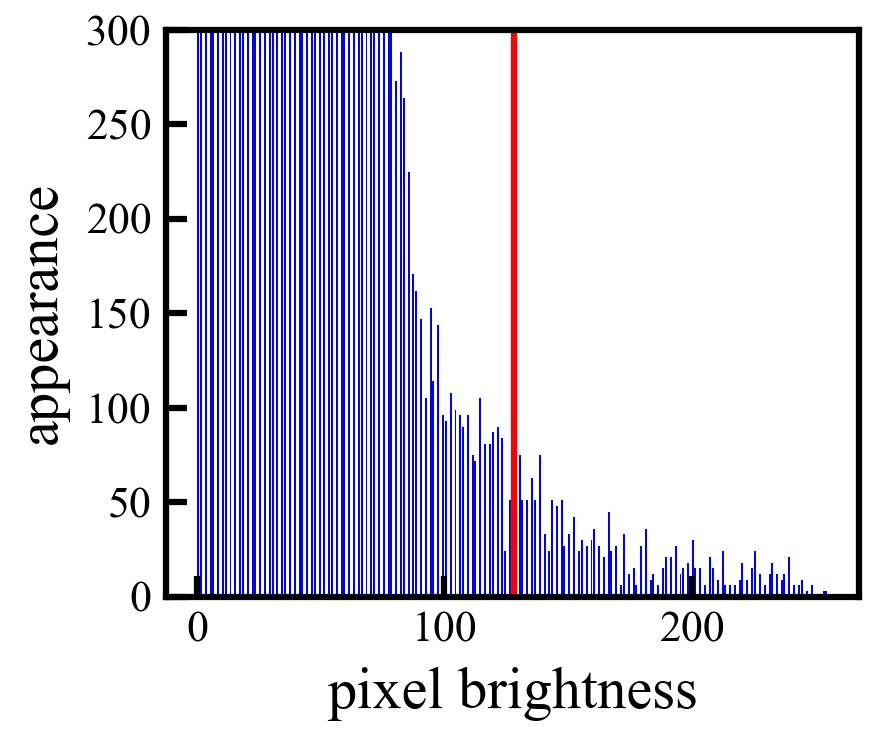
\includegraphics[width=0.98\columnwidth]{./theory/figure/5/thre_norm_hist_2.jpg}
		\end{minipage}
	\end{center}
	\caption{正規化されたヒストグラムにおける閾値(threshold = 128)の設定}
	\label{fig:thre_norm_hist}
\end{figure}

\begin{figure}[h]
	\begin{center}
		\begin{minipage}{0.3\linewidth}
			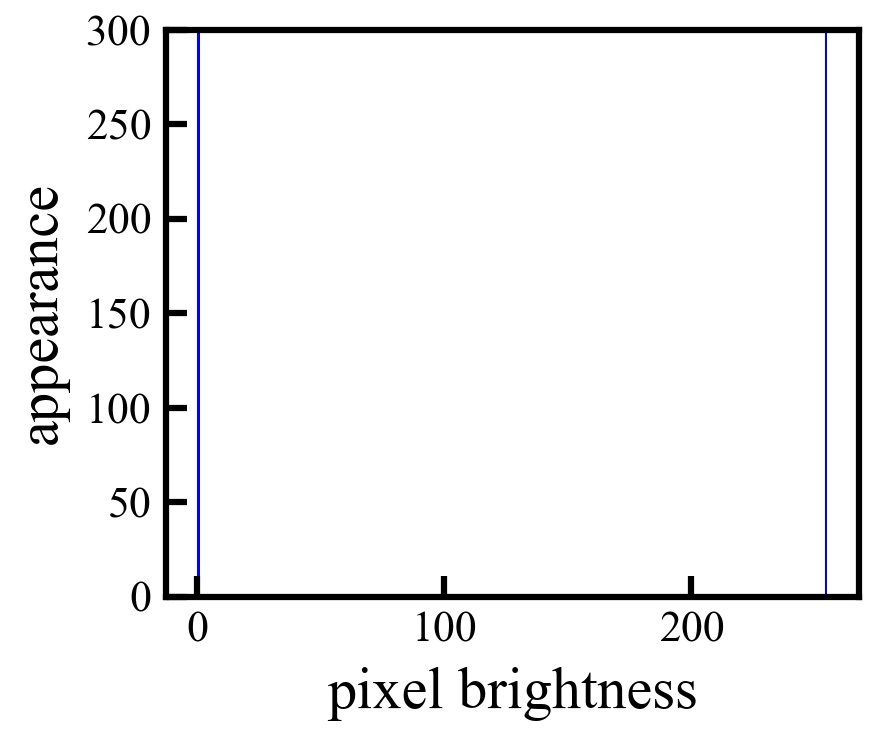
\includegraphics[width=0.98\columnwidth]{./theory/figure/5/binary_0.jpg}
		\end{minipage}
		\begin{minipage}{0.3\linewidth}
			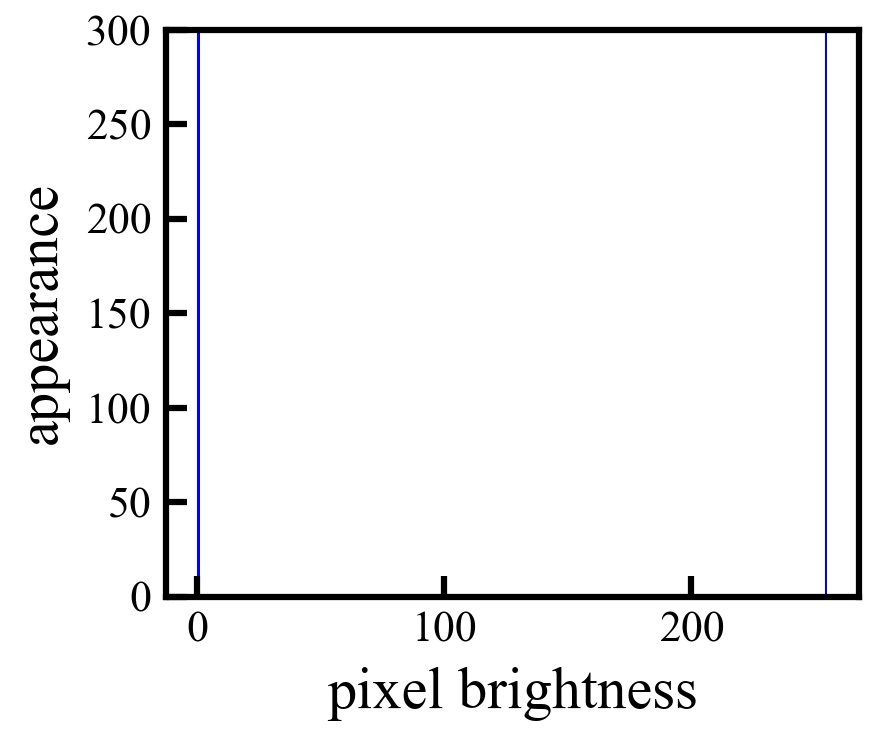
\includegraphics[width=0.98\columnwidth]{./theory/figure/5/binary_1.jpg}
		\end{minipage}
		\begin{minipage}{0.3\linewidth}
			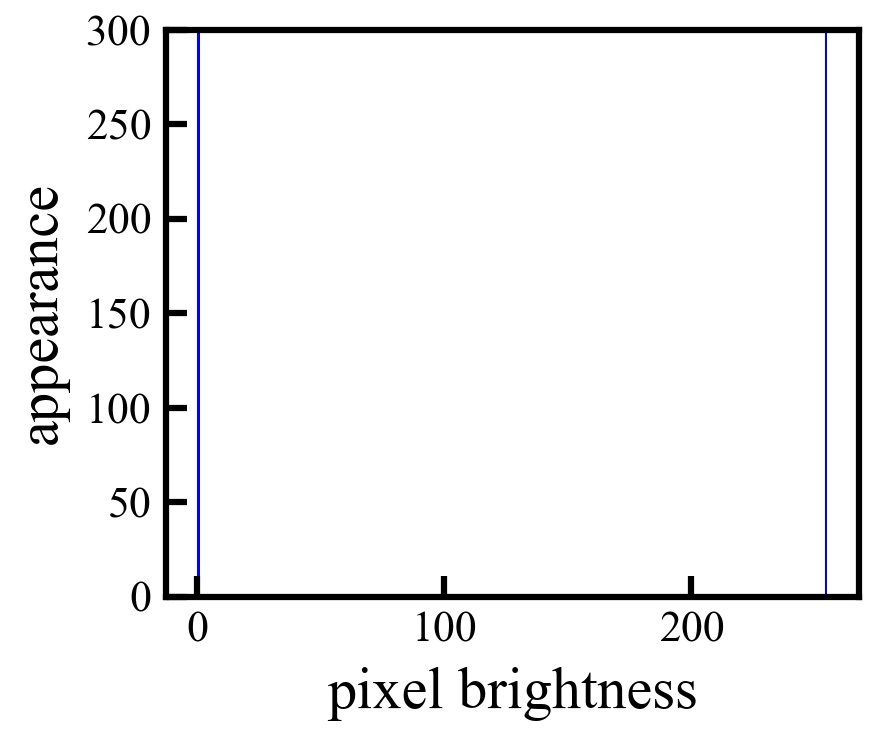
\includegraphics[width=0.98\columnwidth]{./theory/figure/5/binary_2.jpg}
		\end{minipage}
	\end{center}
	\caption{\Fig{thre_norm_hist}に対して,二値化(0,255)の処理を行った後のヒストグラム}
	\label{fig:binary_hist}
\end{figure}

ヒストグラムの正規化を行ったことで,カメラのピントや集光時間およびレーザーの波長や位置の影響を受ける画像の輝度値の二値化が固定の閾値で行うことができる.

\subsection{OpenCVを用いたイオンの検出}
二値化されたイオン捕獲画像において輝度値が255である範囲の面積を求め,ある値以上の面積を持つ範囲をイオンとして計上する.イオンと判定された範囲に対して最小外接円を近似しその中心値をイオンの位置として特定する.

\subsection{電場の算出方法}
イオンの位置を用いて,イオンにかかる電場の算出が可能である.N個のイオンが一列に並んでいるとき,i番目のイオンの座標$z_{i}$における電場$\bm{E}(z_{i})$を求める.イオンが捕獲されている状態では,プレーナートラップが形成する電場から受ける力と他のイオンから受けるクーロン相互作用による力とがつりあっている.したがって,次式が成り立つ\cite{Brownnutt_2012}.
\large
\begin{align}\label{eq:equi_string}
e\bm{E}(z_i) + \frac{e^2}{4\pi \varepsilon_0} \sum^N_{i=0,i\neq j} \frac{z_i - z_j}{|z_i - z_j|^3} = 0.
\end{align}
\normalsize
ここで,$e$は素電荷,$\varepsilon_0$は真空の誘電率を示す.
イオンが二列に並ぶ場合にも,\Eq{equi_string}と同様に平衡の式を満たす.i番目のイオンの位置が($z_i,x_i$)で指定されるとき,
\large
\begin{align}\label{eq:equi_array}
e\bm{E}(z_i,x_i) + \frac{e^2}{4\pi \varepsilon_0}\sum^N_{i=1,i\neq j}\frac{1}{|\bm{r}_{ij}|^2}\frac{\bm{r}_{ij}}{|\bm{r}_{ij}|} = 0,
\end{align}
\normalsize
と書くことができる.ここで,
\large
\begin{align}
\bm{r}_{ij} &= (z_i - z_j)\hat{z} + (x_i - x_j)\hat{x} \notag \\
|\bm{r}_{ij}| &= \sqrt{(z_i - z_j)^2 + (x_i - x_j)^2} \notag 
\end{align}
\normalsize
であり,$\hat{z},\hat{x}$は各軸における単位ベクトルである.また,$\hat{r}_{ij} \equiv \bm{r}_{ij}/|\bm{r}_{ij}|$とすれば,\Eq{equi_array}は,
\large
\begin{align}\label{eq:equi_array_2}
e\bm{E}(z_i,x_i) = \frac{e^2}{4\pi \varepsilon_0}\sum^N_{i=1,i\neq j} \frac{1}{|\bm{r}_{ij}|^2}\hat{r}_{ij} = 0
\end{align}
\normalsize
とまとめられる.二列配列のイオン捕獲位置における電場を導出する際には,\Eq{equi_array_2}を各軸に沿った成分毎に計算を行う.したがって,各成分に分けて書くと,
\large
\begin{align}
eE_z(z_i,x_i) + \frac{e^2}{4\pi \varepsilon_0} \sum^N_{i=1,i \neq j}\frac{z_i - z_j}{|\bm{r}_{ij}|^3} = 0 , \\
eE_x(z_i,x_i) + \frac{e^2}{4\pi \varepsilon_0} \sum^N_{i=1,i \neq j}\frac{x_i - x_j}{|\bm{r}_{ij}|^3} = 0 .
\end{align}
\normalsize
これを解くことで,
\large
\begin{align}
\bm{E}(z,x) = E_z(z,x)\hat{z} + E_x(z,x)\hat{x}
\end{align}
\normalsize
の関係から,イオン捕獲位置における電場の算出を行う.電場の大きさと,z軸からの偏角$\theta$は,
\large
\begin{align}
|\bm{E}(z_i,x_i)| &= \sqrt{E_z^2(z_i,x_i) + E_x^2(z_i,x_i)}, \\
\theta &= \tan^{-1} \left(\frac{E_x(z_i,x_i)}{E_z(z_i,x_i)} \right) .
\end{align}
\normalsize